\begin{figure}[t]
        \begin{subfigure}[b]{0.32\textwidth}
        \centering
        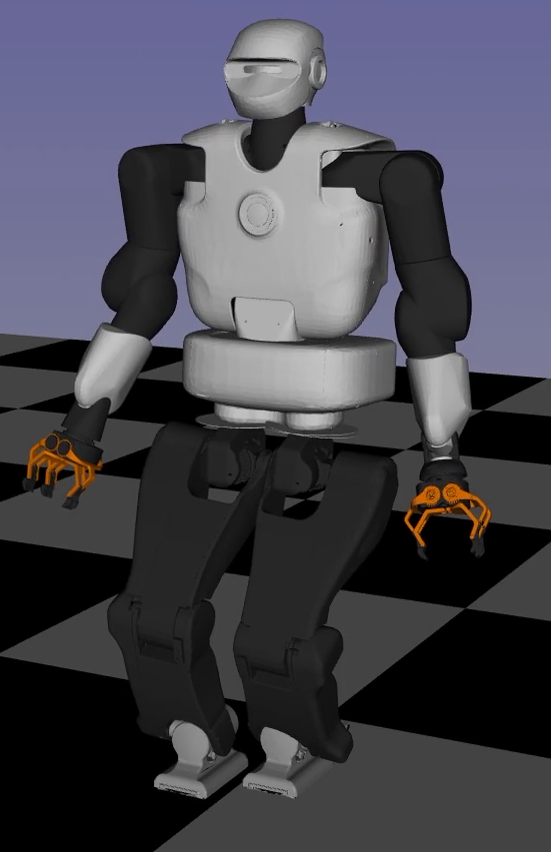
\includegraphics[width=\columnwidth]{chapter_flexible_joints/figures/talos_1.png}
    \end{subfigure}
    \hfill
    \begin{subfigure}[b]{0.32\textwidth}
        \centering
        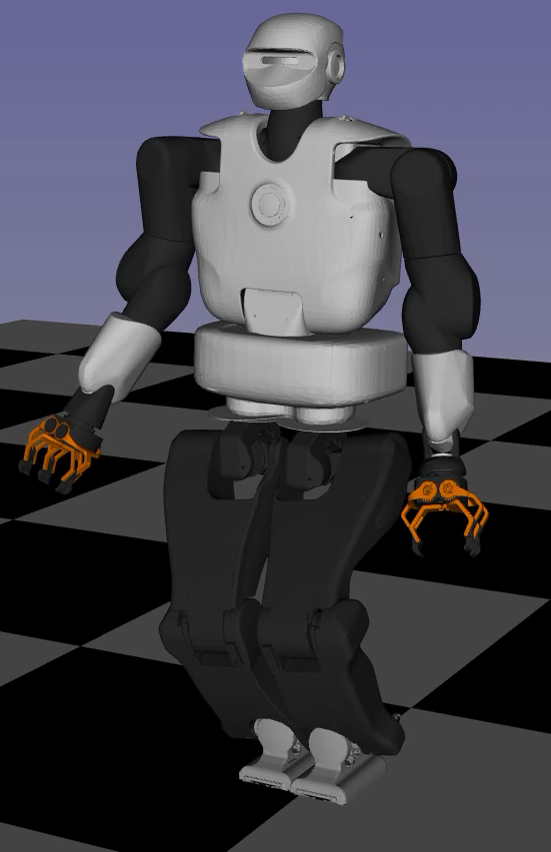
\includegraphics[width=\columnwidth]{chapter_flexible_joints/figures/talos_2.png}
    \end{subfigure}
    \hfill
     \begin{subfigure}[b]{0.32\textwidth}
        \centering
        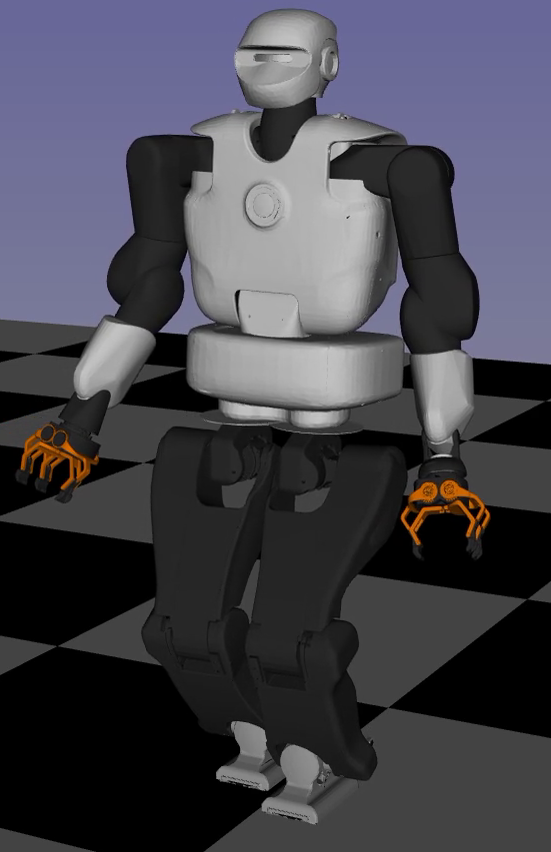
\includegraphics[width=\columnwidth]{chapter_flexible_joints/figures/talos_3.png}
    \end{subfigure}
    \caption{A simulation of the TALOS robot walks with the TSID-Flex controller~\label{fig:talos_flex_walking}}
\end{figure}
\section{Results\label{sec:flexible_joint_result}}
In this section, we present the simulation tests of the control strategy presented in
Section~\ref{sec:wbc_tsid_flex_joints} -- Figure~\ref{fig:talos_flex_walking}.
The proposed control strategy is compared with a whole-body controller that assumes all the robot joints actuated --  see Section~\ref{sec:dynamics_QP}. From now on, the control approach presented in this chapter is called \emph{TSID-Flex} while the controller introduced in Section~\ref{sec:dynamics_QP} \emph{TSID-Rigid}.
The experiments are carried out on a simulated version of the TALOS humanoid robot -- see Section~\ref{sec:talos}. The architecture takes (on average) less than $\SI{1}{\milli \second}$ to evaluate its output. The OSQP~\citep{Stellato2018} library is used to solve the optimization problems. The code is fully implemented in Python~\footnote{The control objective is implemented exploiting the Python bindings provided by the \texttt{bipedal-locomotion-framework} library: \href{https://github.com/ami-iit/bipedal-locomotion-framework/tree/v0.6.0/bindings}{\texttt{https://github.com/ami-iit/bipedal-locomotion-framework/tree/v0.6.0/bindings}}}.
The simulations are obtained by integrating the forward dynamics (FD) of the robot obtained from~\eqref{eq:system_initial}. Figure~\ref{fig:talos_flex_walking_zoom} shows a zoom in on the flexible joints. To simply visualize the link deformation, we introduced two disks with zero masses and zero inertial at the level of the flexibility. When the two disks on the same leg coincide, the positions of the flexible joints are equal to zero.
\par
To validate the performance of the proposed architecture, we present two main experiments.
First, we compare the performance of the TSID-Flex and the TSID-Rigid controllers in the case of different stiffness parameters $k$. Second, we analyze the performance of the TSID-Flex in the case of different stiffness. In both scenarios, the desired robot CoM, footsteps, and actuated joint trajectories are computed offline~\footnote{The whole-body trajectory are provided by: \href{https://github.com/loco-3d/multicontact-api/tree/v2.1.0}{\texttt{https://github.com/loco-3d/multicontact-api/tree/v2.1.0}}}. The robot walks 1 meter forward with a step length of $\SI{20}{\centi\meter}$, starting with the right foot. The first and last steps are $\SI{10}{\centi \meter}$ long. The double support lasts $\SI{0.2}{\second}$, while the single support lasts $\SI{1.2}{\second}$.
\begin{figure}[t]
        \begin{subfigure}[b]{0.32\textwidth}
        \centering
        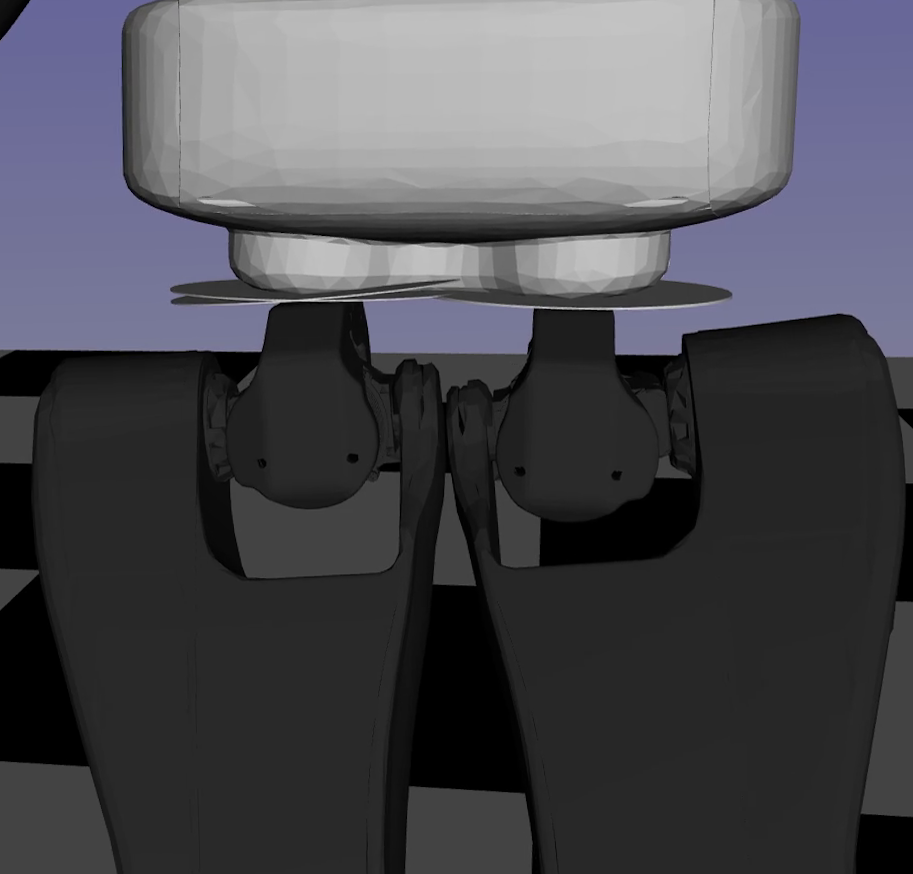
\includegraphics[width=\columnwidth]{chapter_flexible_joints/figures/zoom_flex_1.png}
    \end{subfigure}
    \hfill
    \begin{subfigure}[b]{0.32\textwidth}
        \centering
        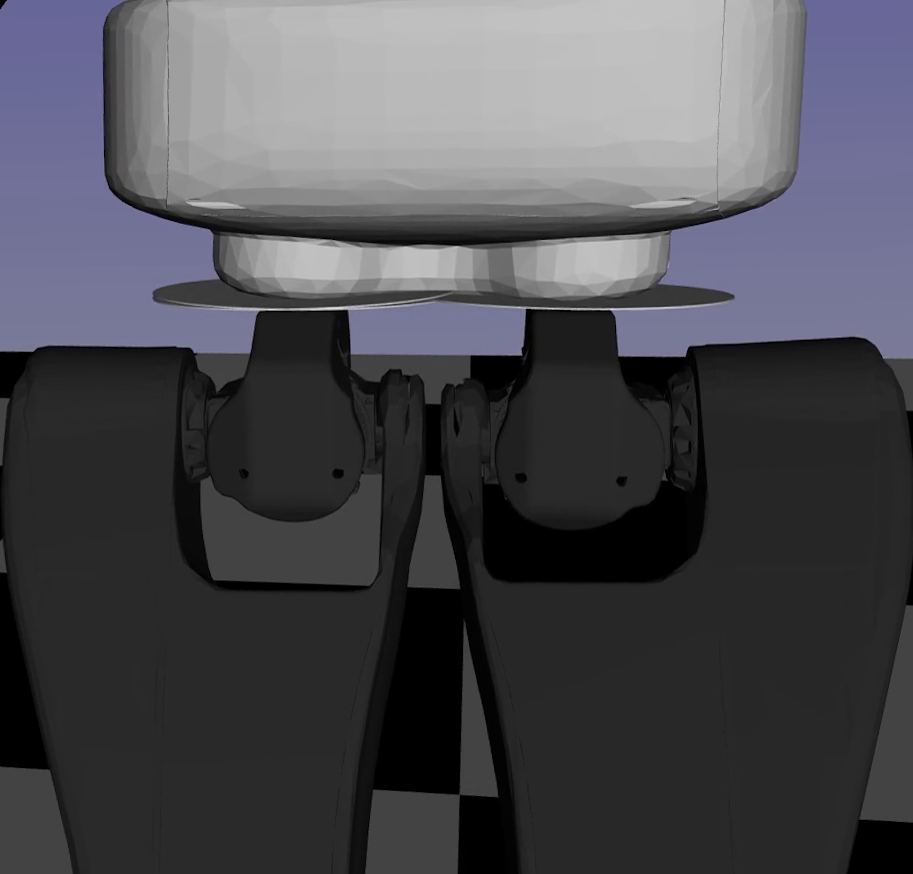
\includegraphics[width=\columnwidth]{chapter_flexible_joints/figures/zoom_flex_2.png}
    \end{subfigure}
    \hfill
     \begin{subfigure}[b]{0.32\textwidth}
        \centering
        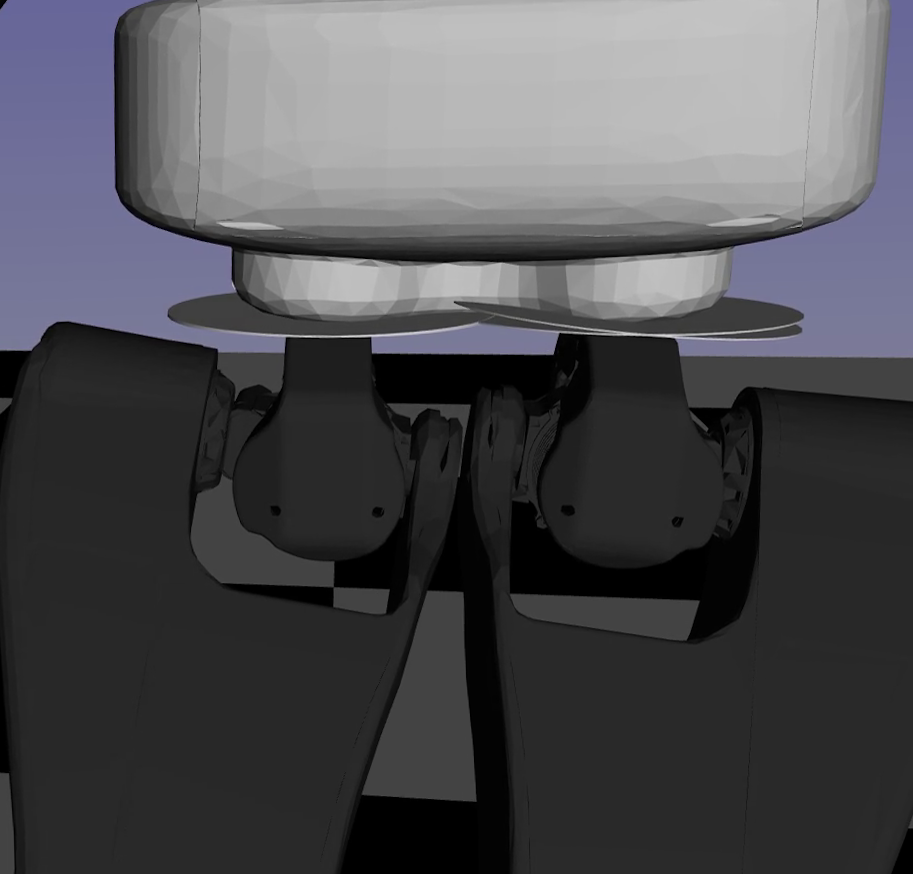
\includegraphics[width=\columnwidth]{chapter_flexible_joints/figures/zoom_flex_3.png}
    \end{subfigure}
    \caption{Zoom of the flexible joints motion\label{fig:talos_flex_walking_zoom}.}
\end{figure}
\begin{figure}[!t]
    \begin{myframe}{k = $\SI{1e4}{\newton \per \radian}$}
    \centering
        \begin{subfigure}[b]{0.49\textwidth}
        \centering
        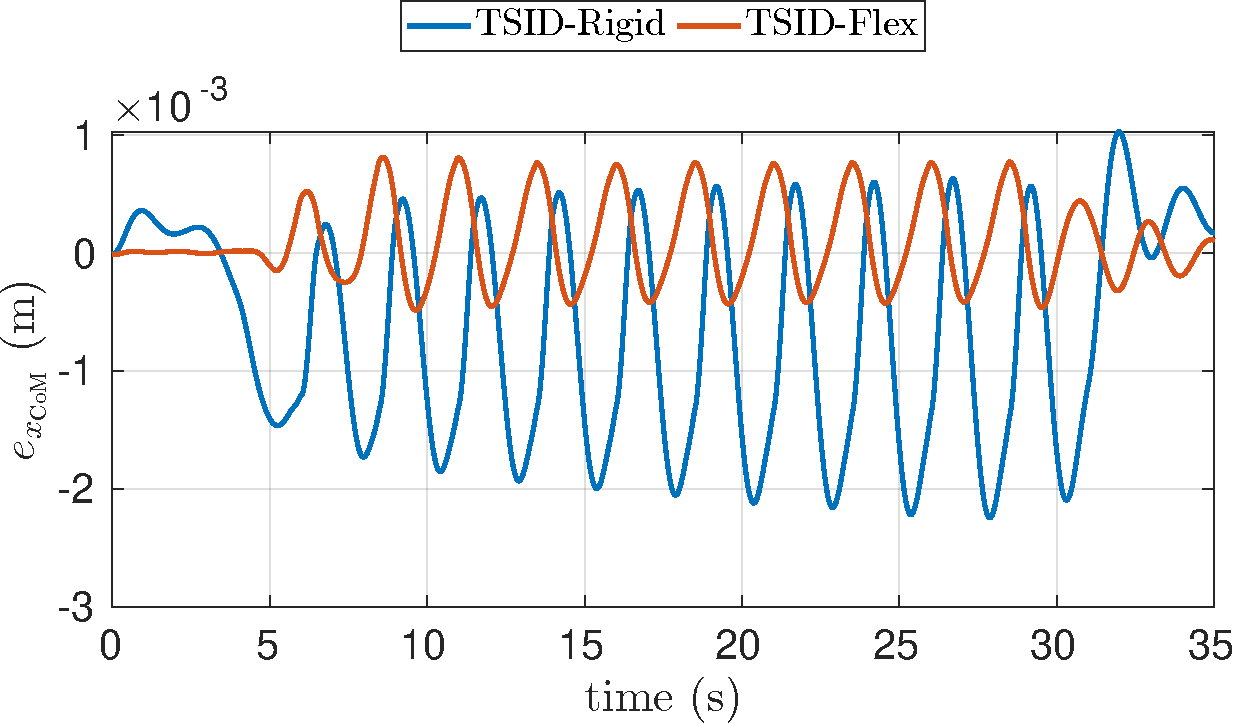
\includegraphics[width=\columnwidth]{chapter_flexible_joints/figures/comparison_10000_com_error_x.pdf}
        \caption{CoM - x}
    \end{subfigure}
    \hfill
    \begin{subfigure}[b]{0.49\textwidth}
        \centering
        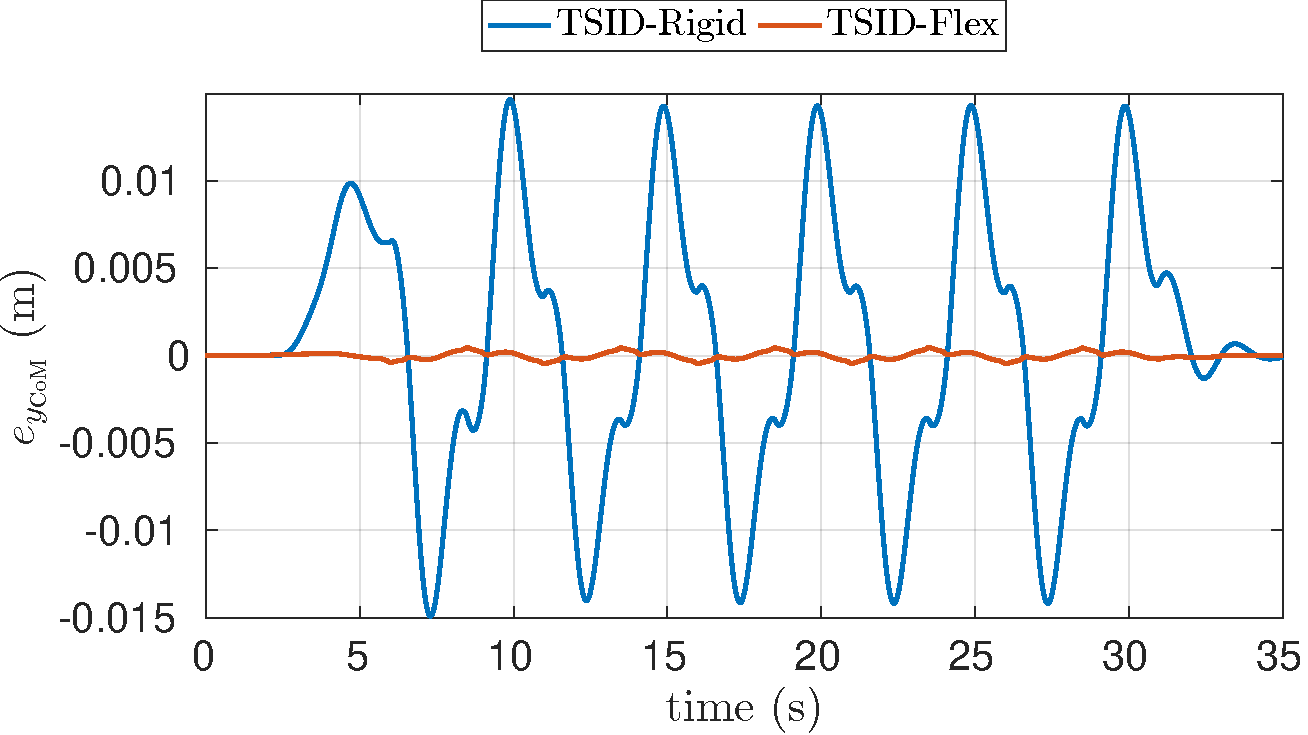
\includegraphics[width=\columnwidth]{chapter_flexible_joints/figures/comparison_10000_com_error_y.pdf}
        \caption{CoM - y}
    \end{subfigure}
     \begin{subfigure}[b]{0.49\textwidth}
        \centering
        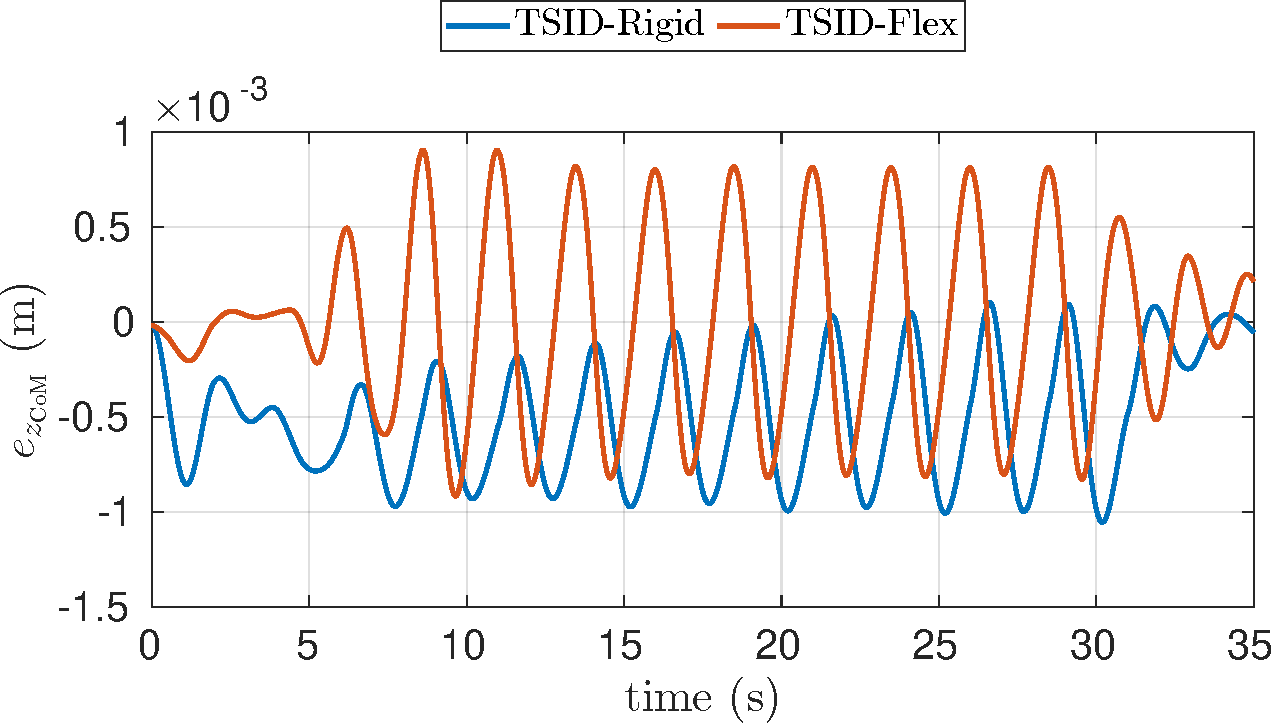
\includegraphics[width=\columnwidth]{chapter_flexible_joints/figures/comparison_10000_com_error_z.pdf}
        \caption{CoM - z}
    \end{subfigure}
    \end{myframe}
    \caption{CoM tracking: comparison between TSID-Rigid and TSID-Flex.\label{fig:com_tracking_10000_com_rigid_flex}}
\end{figure}
\begin{figure}[t]
    \begin{myframe}{k = $\SI{1e4}{\newton \per \radian}$}
    \centering
        \begin{subfigure}[b]{0.49\textwidth}
        \centering
        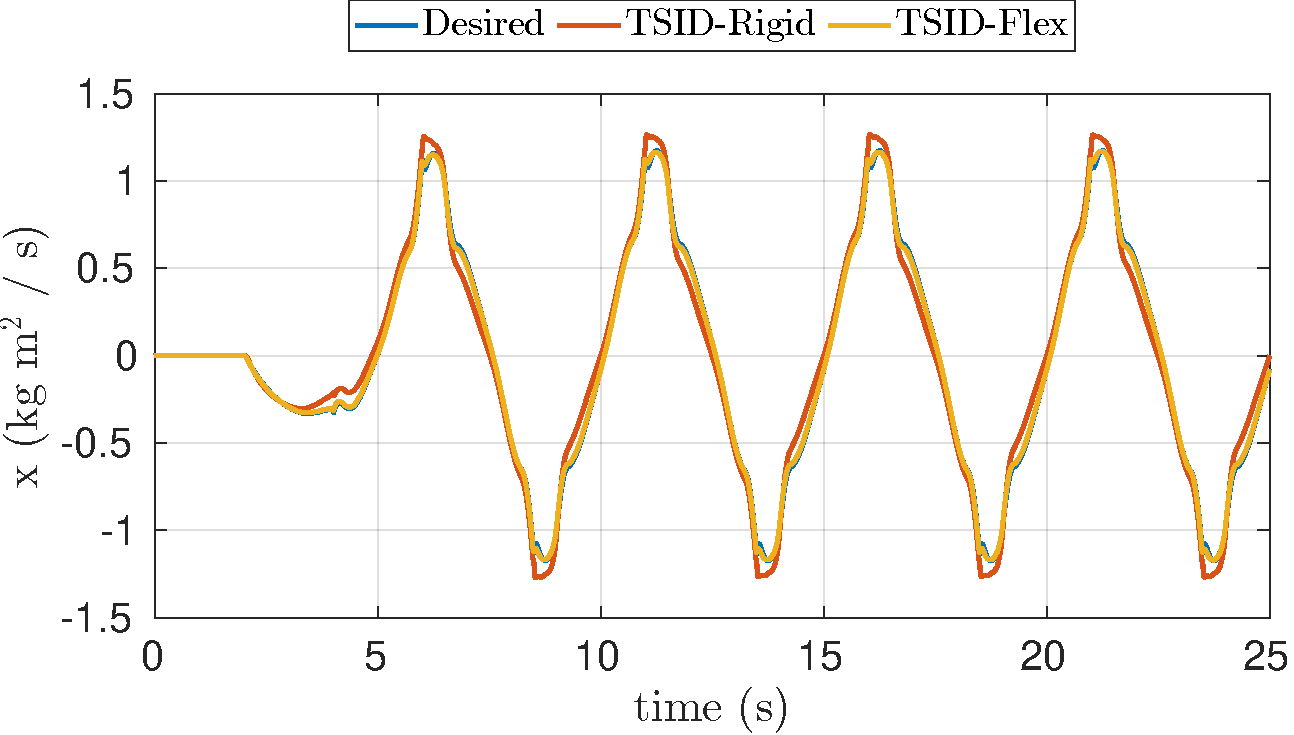
\includegraphics[width=\columnwidth]{chapter_flexible_joints/figures/comparison_10000_angular_momentum_x.pdf}
        \caption{Angular Momentum - x}
    \end{subfigure}
    \hfill
    \begin{subfigure}[b]{0.49\textwidth}
        \centering
        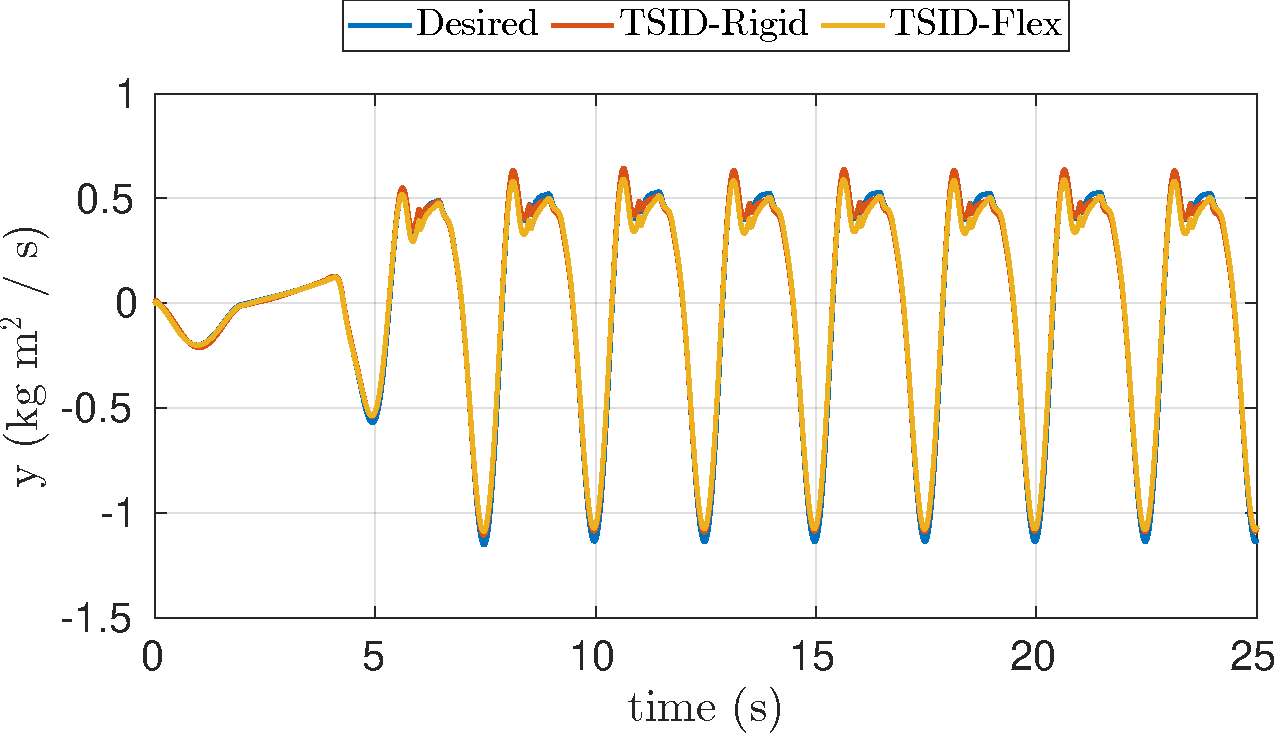
\includegraphics[width=\columnwidth]{chapter_flexible_joints/figures/comparison_10000_angular_momentum_y.pdf}
        \caption{Angular Momentum - y}
    \end{subfigure}
     \begin{subfigure}[b]{0.49\textwidth}
        \centering
        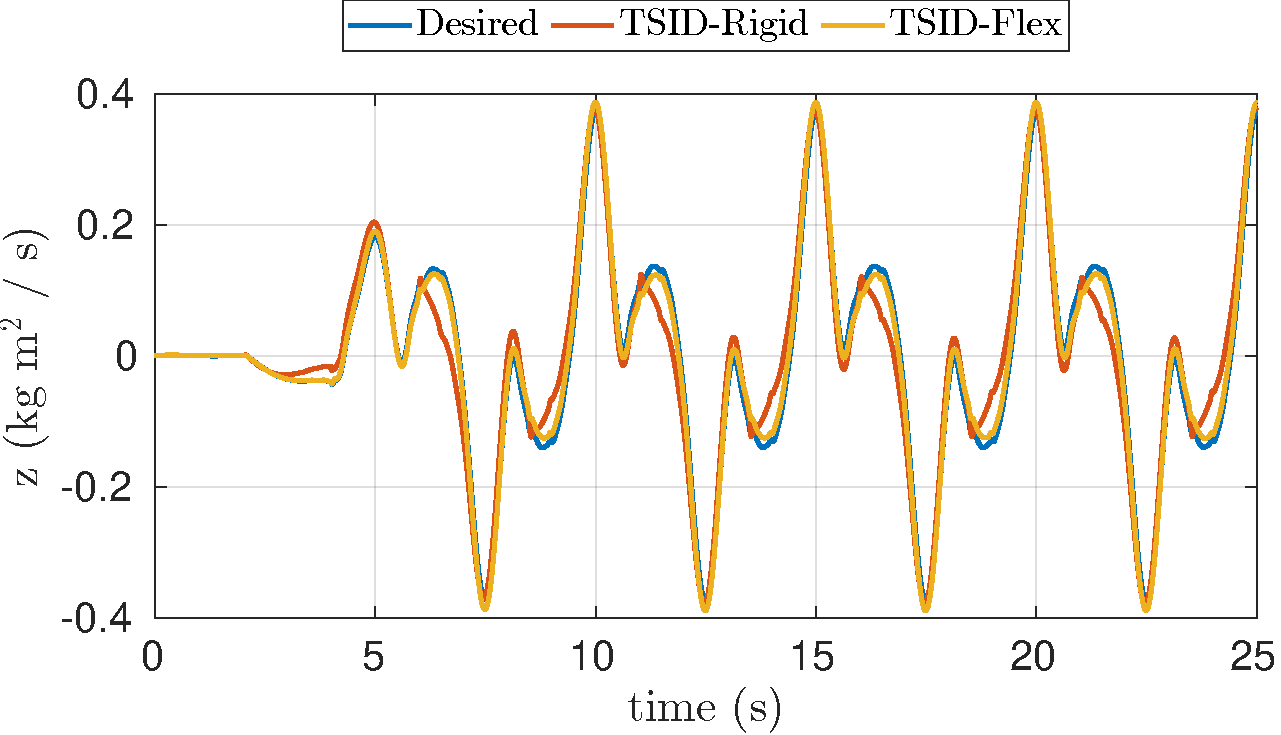
\includegraphics[width=\columnwidth]{chapter_flexible_joints/figures/comparison_10000_angular_momentum_z.pdf}
        \caption{Angular Momentum - z}
    \end{subfigure}
    \end{myframe}
    \caption{Angular momentum tracking: comparison between TSID-Rigid and TSID-Flex.\label{fig:angular_momentum_tracking_10000_rigid_flex}}
\end{figure}

\subsection{Comparison between TSID-Flex and TSID-Rigid}
In Table~\ref{tab:flex_joint_architecture_outcome}, we summarize the results of the control strategies for different stiffness parameters $k$. The labels \emph{success} and \emph{failure} mean that the associated controller is either able or not to ensure the robot's balance while walking. In all the experiments presented in this section, the damping parameter is arbitrarily set to $b=2\sqrt{k}$. 
\par
\begin{table}[b]
    \centering
    \caption[Controllers outcome in the case of different joint stiffness parameter $k$]{Controller implementation outcome in the case of different joint stiffness parameter $k$. The damping parameter is set to $b=2\sqrt{k}$. 
    }
    \begin{tabular}{c|ccccc}
         Whole-Body Control &
         $\SI{10}{\kilo\newton\per\radian}$ & $\SI{5}{\kilo \newton\per\radian}$&$\SI{3}{\kilo \newton\per\radian}$& $\SI{2}{\kilo \newton\per\radian}$& $\SI{1}{\kilo \newton\per\radian}$  \\
        \hline
        TSID-Rigid  & success  &  success & failure& failure& failure\\
        TSID-Flex  & success  & success & success  & success & success  
    \end{tabular}
    \label{tab:flex_joint_architecture_outcome}
\end{table}
To compare the two controllers, we decided to perform two main experiments. In the former, we choose a set of flexible parameters such that both whole-body controllers guarantee the balance while walking. In the latter, we decrease the value of the stiffness parameter. Namely: 
\begin{itemize}
    \item[\textbf{-}]\textbf{Experiment 1} $k=\SI{1e4}{\newton \per \radian}$;
    \item[\textbf{-}]\textbf{Experiment 2} $k=\SI{3e3}{\newton \per \radian}$.
\end{itemize}

\subsubsection{Experiment 1}
Figure~\ref{fig:com_tracking_10000_com_rigid_flex} shows the CoM tracking performance obtained with TSID-Flex and TSID-Rigid in terms of tracking error. The TSID-Flex controller seems to show good tracking performance and the CoM error is kept below $\SI{2}{\milli \meter}$. On the other hand, the TSID-Rigid induces a higher error on the CoM tracking.
Similar considerations hold also for the tracking of the centroidal angular momentum.

\begin{figure}[!t]
    \begin{myframe}{k = $\SI{1e4}{\newton \per \radian}$}
    \centering
        \begin{subfigure}[b]{0.49\textwidth}
        \centering
        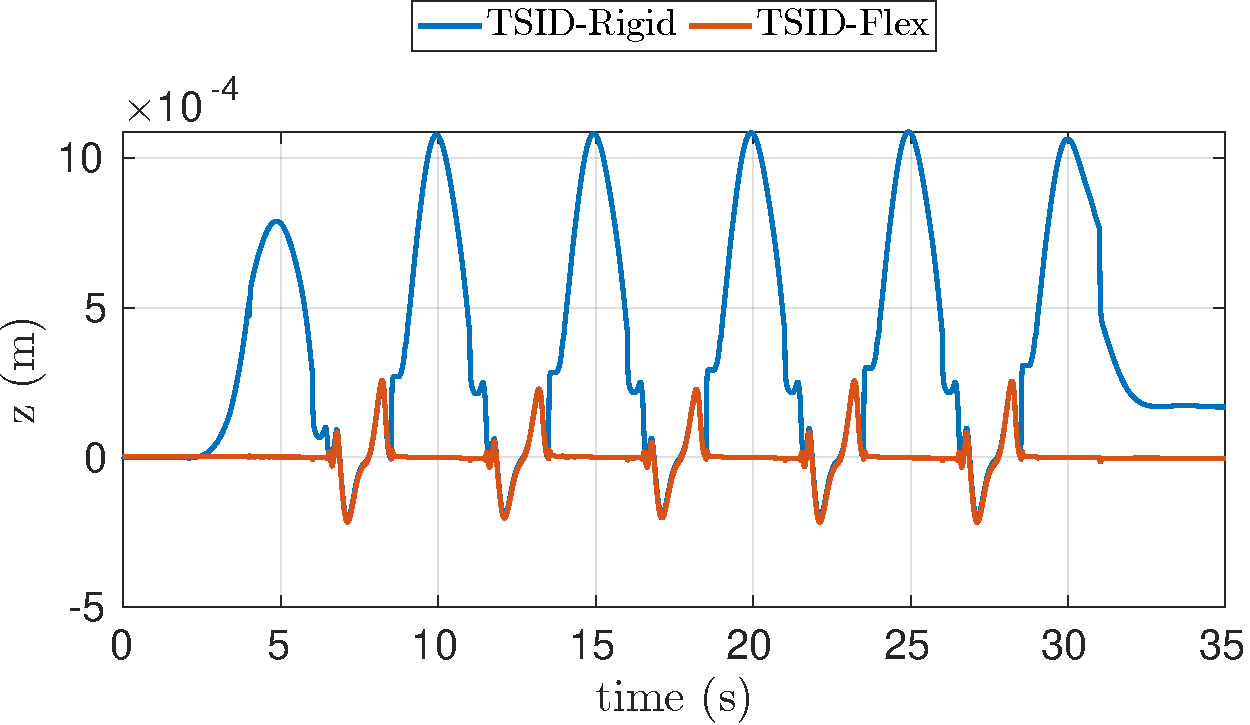
\includegraphics[width=\columnwidth]{chapter_flexible_joints/figures/comparison_10000_left_foot_position_error_z.pdf}
        \caption{Foot tracking position error - z}
    \end{subfigure}
    \hfill
    \begin{subfigure}[b]{0.49\textwidth}
        \centering
        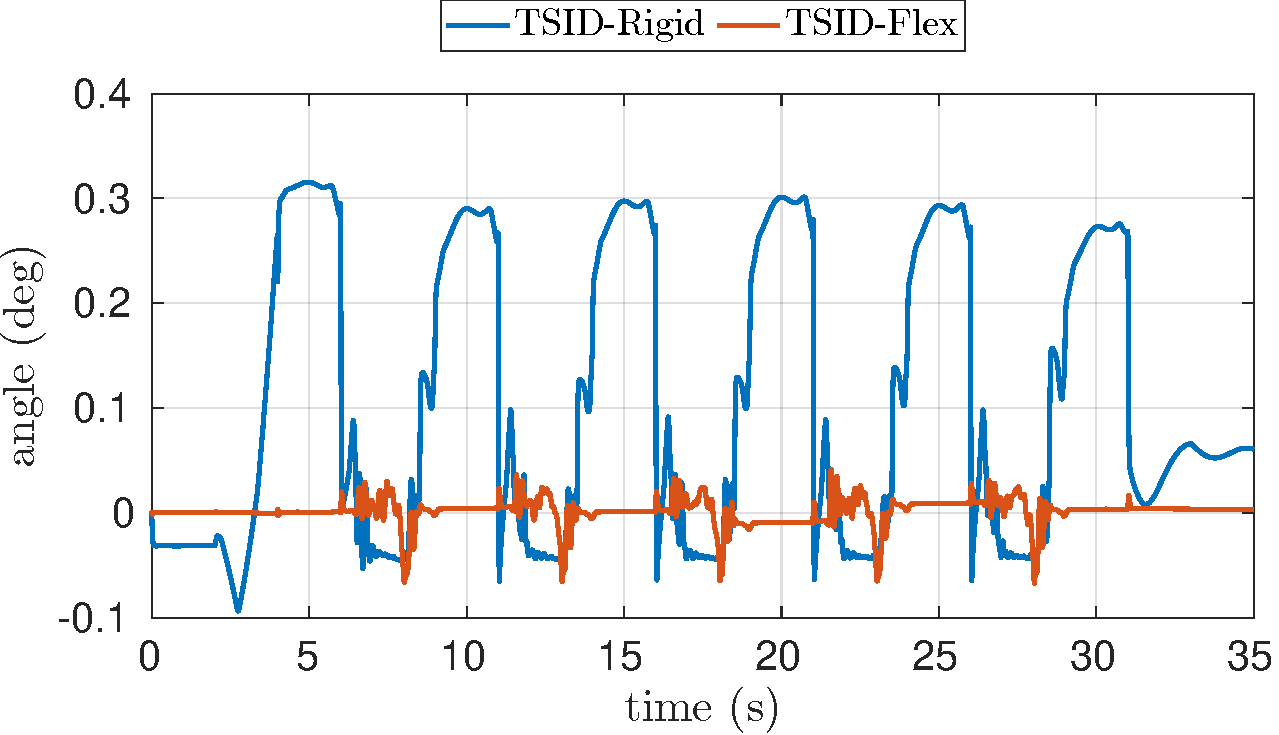
\includegraphics[width=\columnwidth]{chapter_flexible_joints/figures/comparison_10000_left_foot_angle_rot_error.pdf}
        \caption{Foot tracking angular error}
    \end{subfigure}
    \end{myframe}
    \caption{Foot tracking: comparison between TSID-Rigid and TSID-Flex.\label{fig:foot_error_10000_rigid_flex}}
\end{figure}
Figure~\ref{fig:angular_momentum_tracking_10000_rigid_flex} presents the tracking of the angular momentum. The TSID-Flex ensures a smaller angular momentum error with respect to the TSID-Rigid. 
One reason for this behavior is that the TSID-Rigid assumes full control of all the robot joints. This assumption is generally valid in the case of stiff $k$, but it does not hold if $k$ decreases. Figure~\ref{fig:foot_error_10000_rigid_flex} presents the left foot trajectory error when the whole-body controller is TSID-Flex or TSID-Rigid. The angular error is given by the angle of the axis-angle representation between the foot orientation and the desired orientation~\citep{Huynh2009}. Since TSID-Rigid does not consider flexible joint deformation, the controller assumes a wrong foot orientation when the robot is on single support -- for $ \SI{2.5}{\second} \le t \le  \SI{5.5}{\second}$ in Figure~\ref{fig:foot_error_10000_rigid_flex}.


\begin{figure}[t]
    \begin{myframe}{k = $\SI{3e3}{\newton \per \radian}$}
    \centering
        \begin{subfigure}[b]{0.49\textwidth}
        \centering
        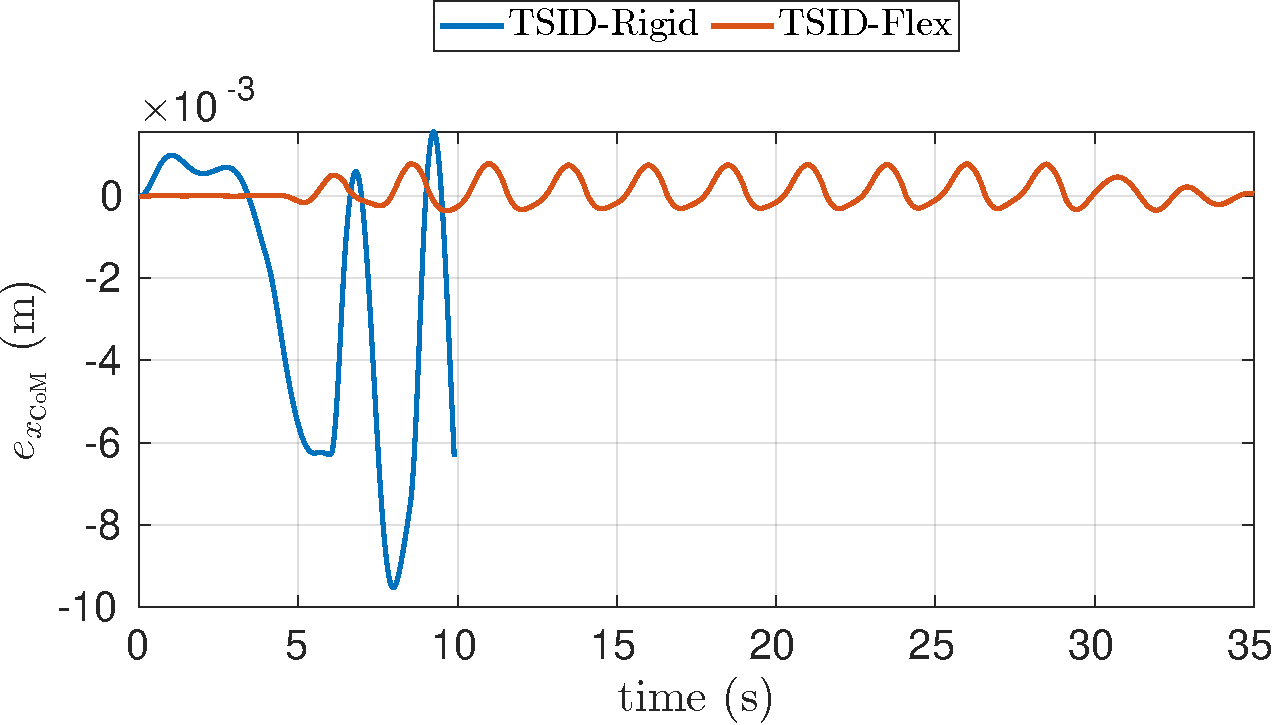
\includegraphics[width=\columnwidth]{chapter_flexible_joints/figures/comparison_3000_com_error_x.pdf}
        \caption{CoM - x}
    \end{subfigure}
    \hfill
    \begin{subfigure}[b]{0.49\textwidth}
        \centering
        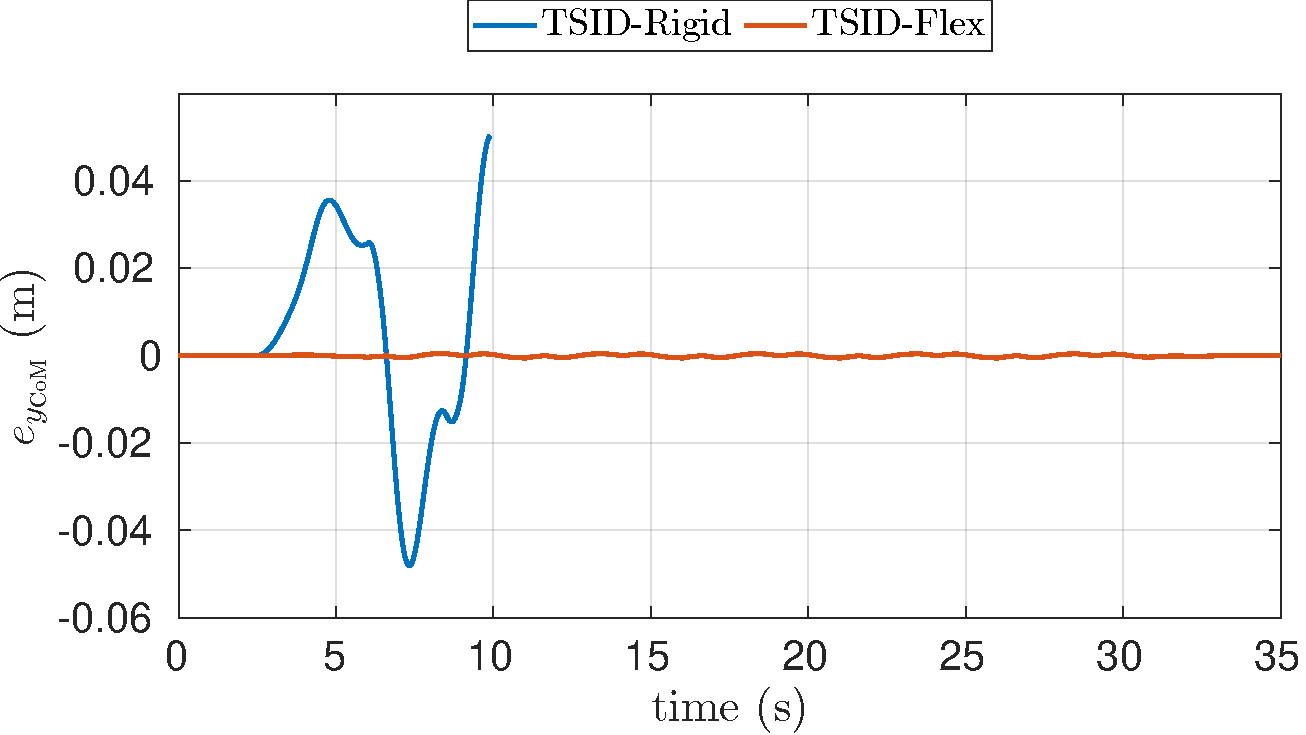
\includegraphics[width=\columnwidth]{chapter_flexible_joints/figures/comparison_3000_com_error_y.pdf}
        \caption{CoM - y}
    \end{subfigure}
     \begin{subfigure}[b]{0.49\textwidth}
        \centering
        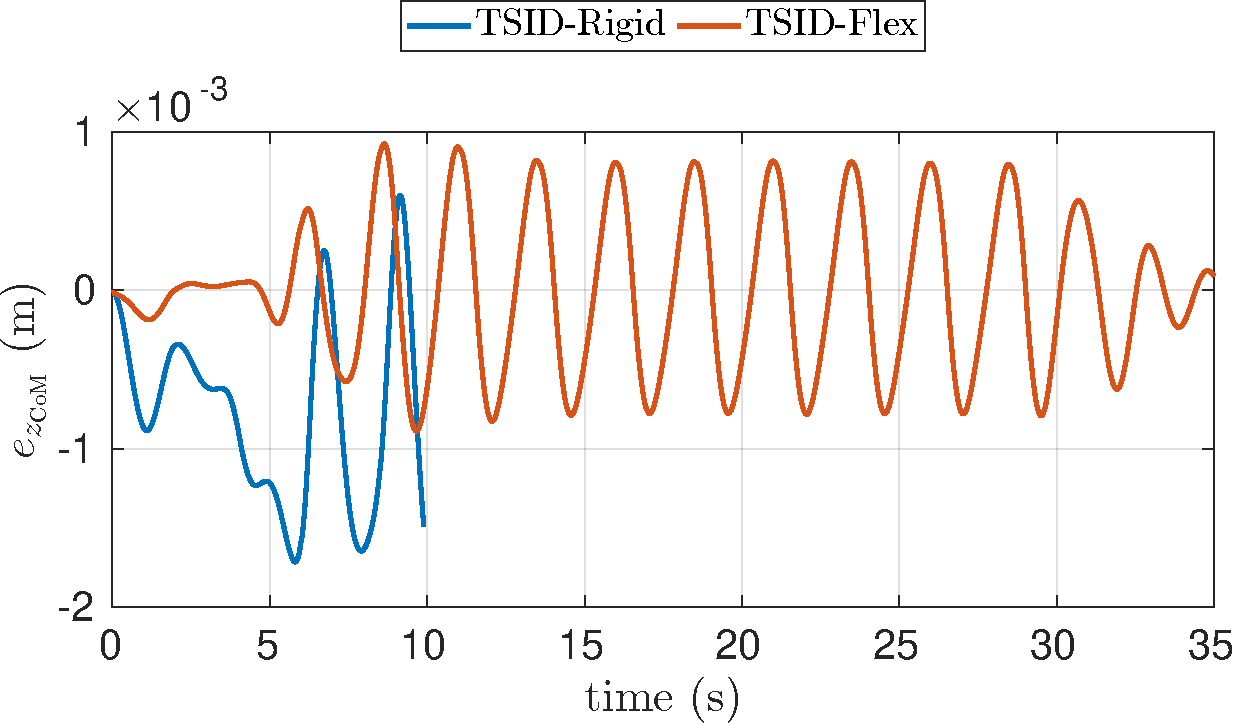
\includegraphics[width=\columnwidth]{chapter_flexible_joints/figures/comparison_3000_com_error_z.pdf}
        \caption{CoM - z}
    \end{subfigure}
    \end{myframe}
    \caption{CoM tracking: comparison between TSID-Rigid and TSID-Flex.\label{fig:com_tracking_3000_com_rigid_flex}}
\end{figure}


\subsubsection{Experiment 2}
The centroidal quantity tracking issue discussed in Experiment 1 worsens at lower values of the stiffness parameter $k$.
Figure~\ref{fig:com_tracking_3000_com_rigid_flex} shows the CoM tracking performances of the two controllers. In Figure~\ref{fig:angular_momentum_tracking_3000_rigid_flex} we present the tracking of the angular momentum. The TSID-Flex is still capable of ensuring good performance. On the other hand, the TSID-Rigid does not consider the flexible joint state. As a consequence, this leads to a non-negligible error on the robot CoM. In order to keep the balance, the TSID-Rigid controller requires high variations of the robot's foot orientation -- see Figure~\ref{fig:foot_error_3000_rigid_flex}. At $t\approx\SI{10}{\second}$ the robot falls.

\begin{figure}[p]
    \begin{myframe}{k = $\SI{3e3}{\newton \per \radian}$}
    \centering
        \begin{subfigure}[b]{0.49\textwidth}
        \centering
        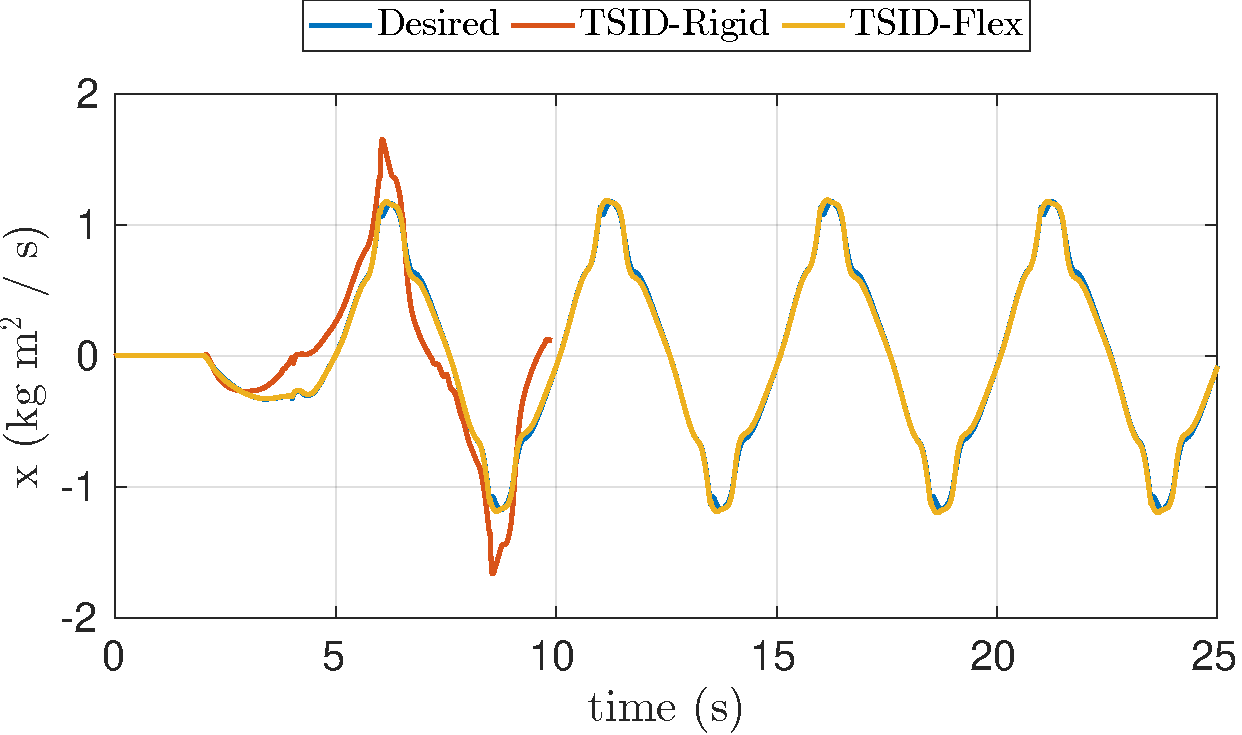
\includegraphics[width=\columnwidth]{chapter_flexible_joints/figures/comparison_3000_angular_momentum_x.pdf}
        \caption{Angular Momentum - x}
    \end{subfigure}
    \hfill
    \begin{subfigure}[b]{0.49\textwidth}
        \centering
        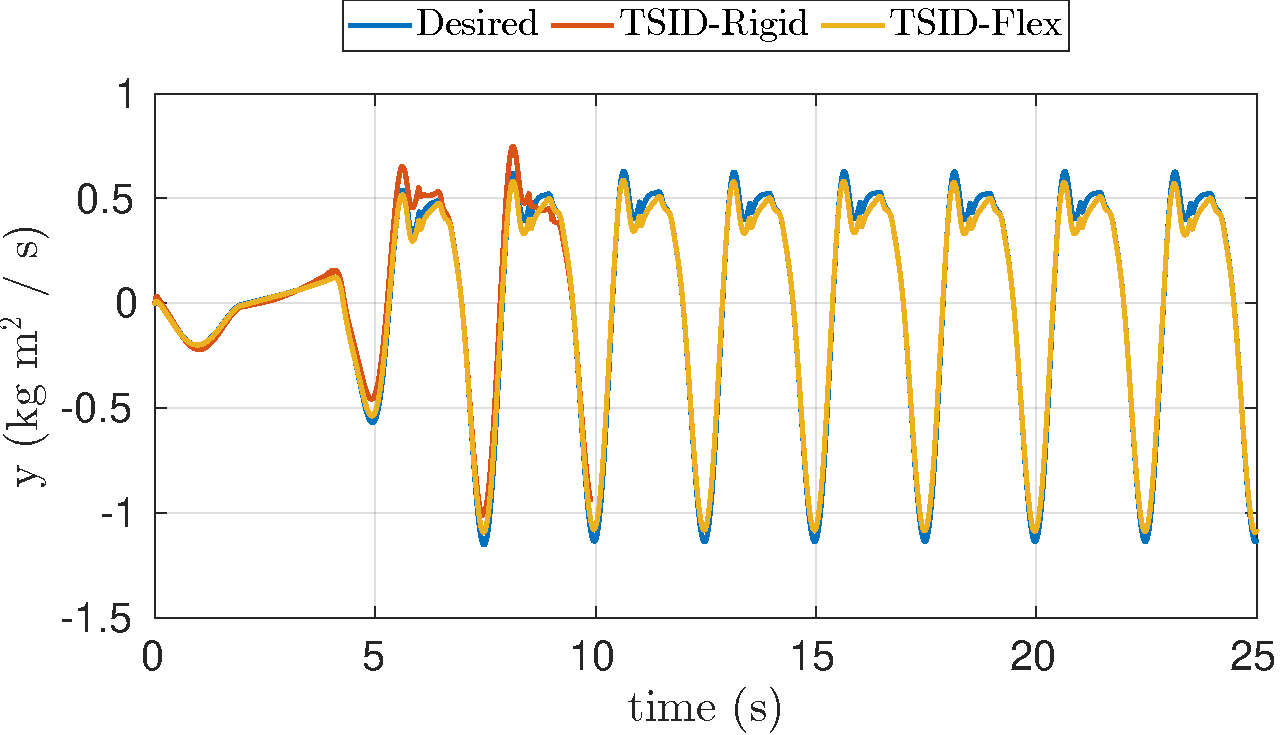
\includegraphics[width=\columnwidth]{chapter_flexible_joints/figures/comparison_3000_angular_momentum_y.pdf}
        \caption{Angular Momentum - y}
    \end{subfigure}
     \begin{subfigure}[b]{0.49\textwidth}
        \centering
        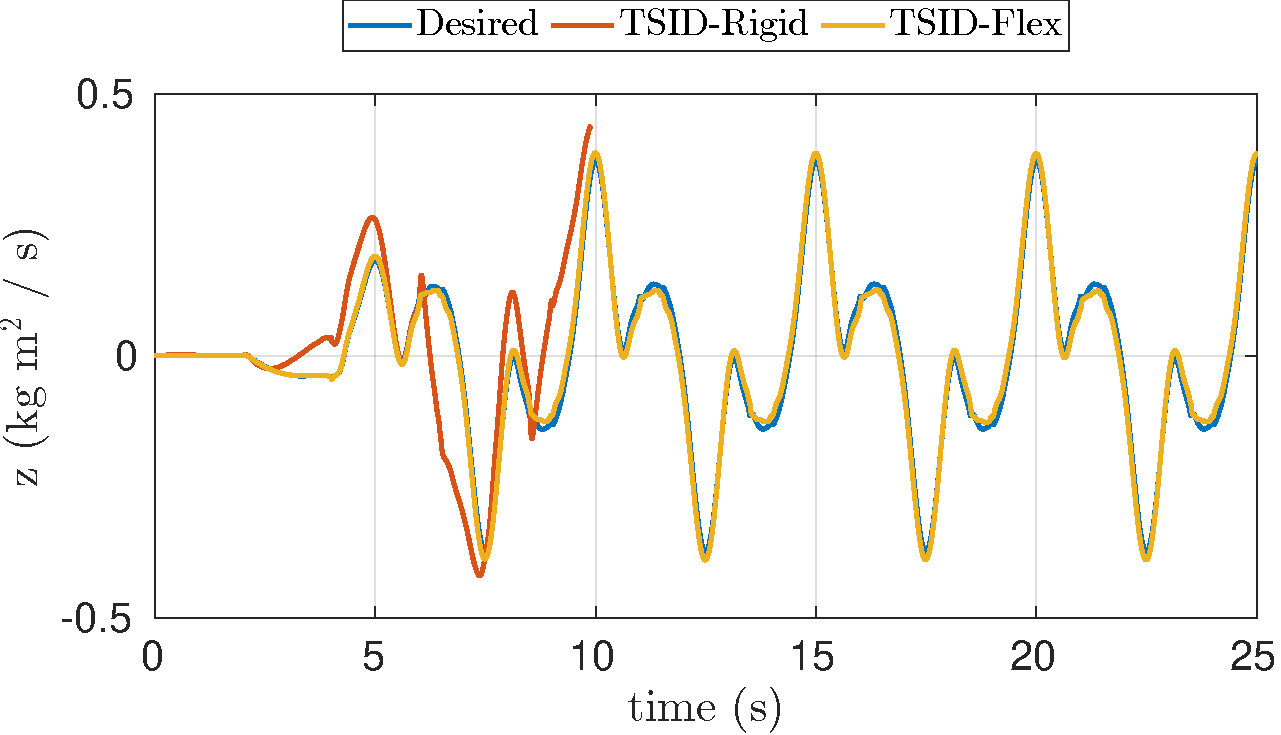
\includegraphics[width=\columnwidth]{chapter_flexible_joints/figures/comparison_3000_angular_momentum_z.pdf}
        \caption{Angular Momentum - z}
    \end{subfigure}
    \end{myframe}
    \caption{Angular momentum tracking: comparison between TSID-Rigid and TSID-Flex.\label{fig:angular_momentum_tracking_3000_rigid_flex}}
\end{figure}

\begin{figure}[p]
    \begin{myframe}{k = $\SI{3e3}{\newton \per \radian}$}
    \centering
        \begin{subfigure}[b]{0.49\textwidth}
        \centering
        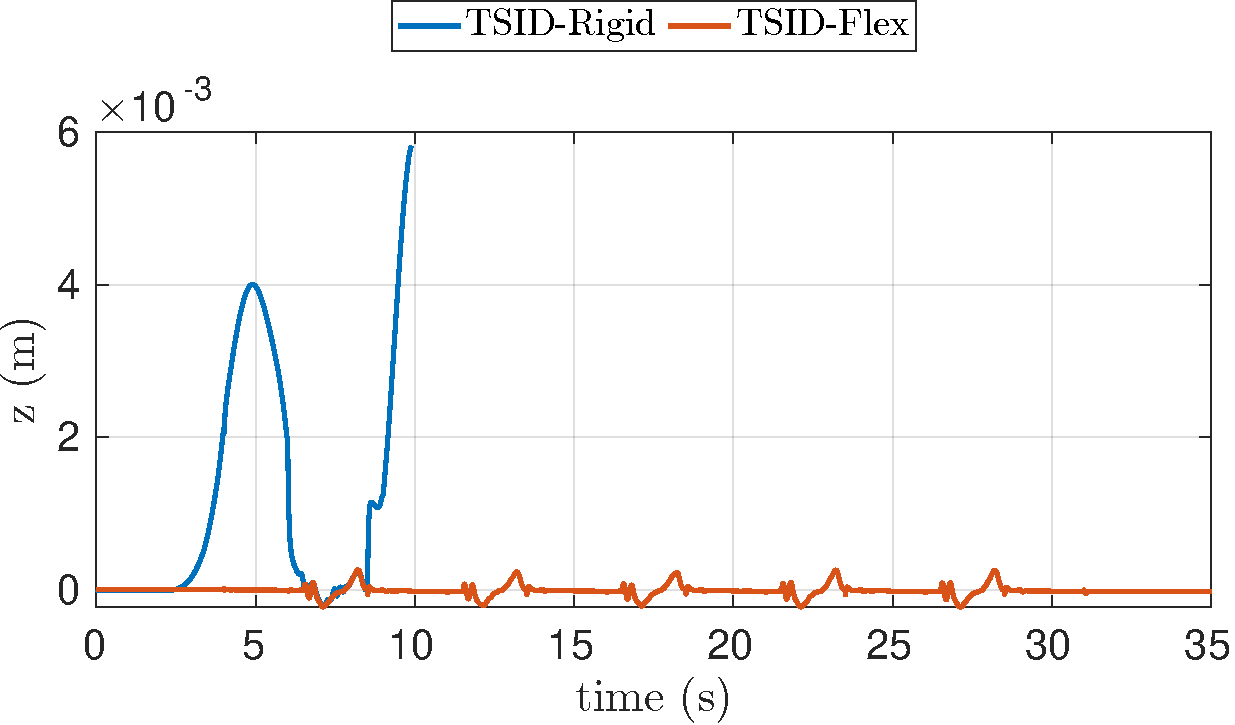
\includegraphics[width=\columnwidth]{chapter_flexible_joints/figures/comparison_3000_left_foot_position_error_z.pdf}
        \caption{Foot tracking position error - z}
    \end{subfigure}
    \hfill
    \begin{subfigure}[b]{0.49\textwidth}
        \centering
        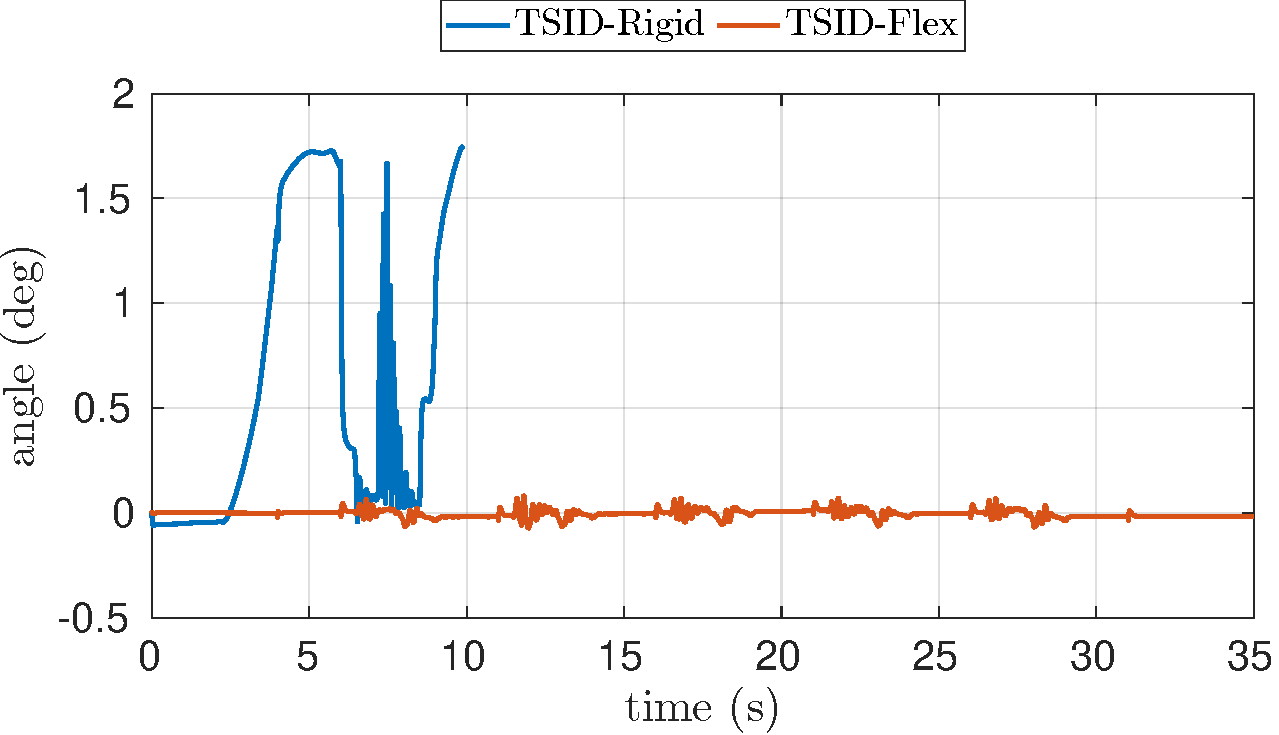
\includegraphics[width=\columnwidth]{chapter_flexible_joints/figures/comparison_3000_left_foot_angle_rot_error.pdf}
        \caption{Foot tracking angular error}
    \end{subfigure}
    \end{myframe}
    \caption{Foot tracking: comparison between TSID-Rigid and TSID-Flex.\label{fig:foot_error_3000_rigid_flex}}
\end{figure}


\subsection{Performances of the TSID-Flex in the case of different stiffness parameters}

In this section, we benchmark the performance of the TSID-Flex controller in the case of different stiffness parameter $k$, namely $k= \SI{10}{\kilo \newton\per\radian}$, $\SI{5}{\kilo \newton\per\radian}$, $\SI{3}{\kilo \newton\per\radian}$, $\SI{2}{\kilo \newton\per\radian}$, $\SI{1}{\kilo \newton\per\radian}$, and $\SI{0.5}{\kilo \newton\per\radian}$.  In all experiments presented in this section, the damping parameter is arbitrarily set to $b=2\sqrt{k}$.

\begin{figure}[t]
    \begin{myframe}{TSID-Flex performances in the case of different $k$}
    \centering
        \begin{subfigure}[b]{0.8\textwidth}
        \centering
        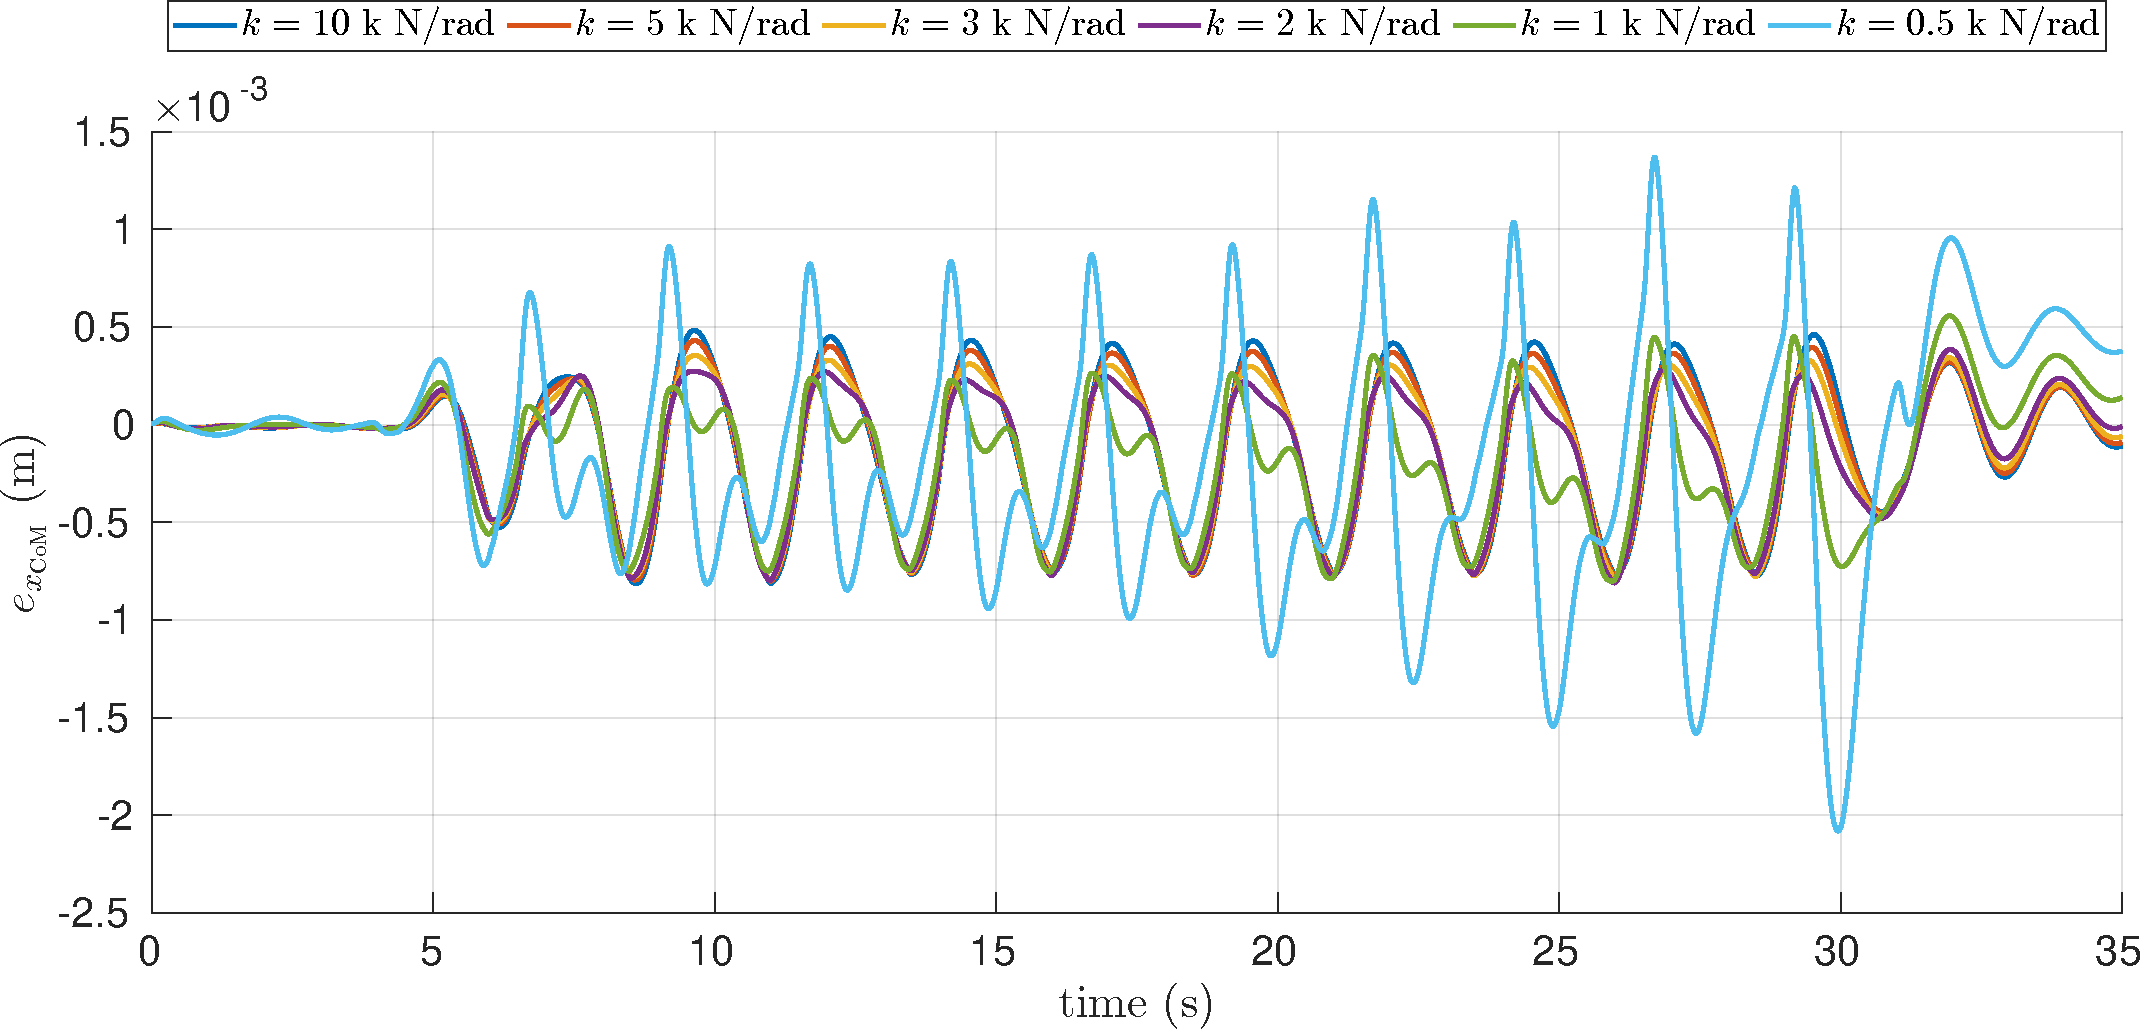
\includegraphics[width=\columnwidth]{chapter_flexible_joints/figures/estimation_com_x_flex.pdf}
        \caption{CoM x error.\label{fig:estimation_com_x_flex}}
    \end{subfigure}
    \hfill
    \begin{subfigure}[b]{0.8\textwidth}
        \centering
        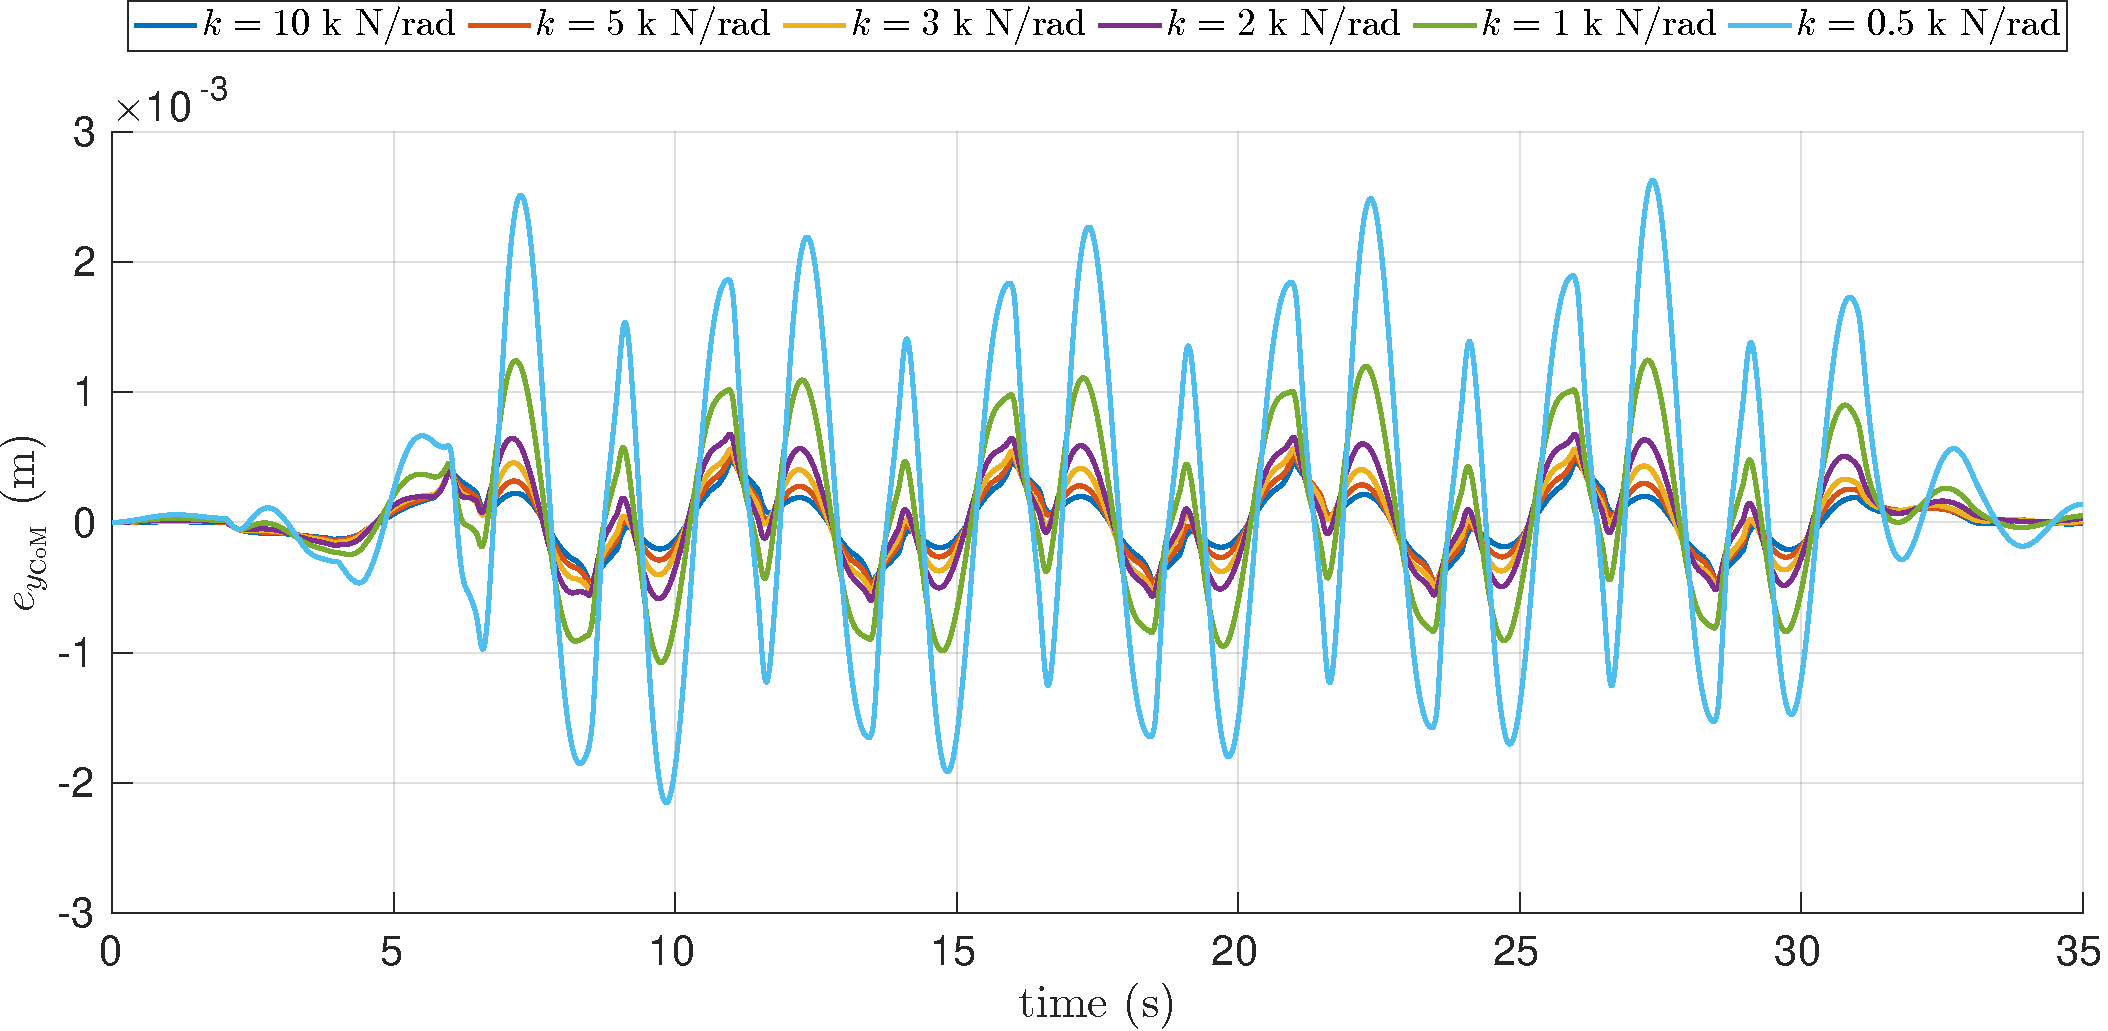
\includegraphics[width=\columnwidth]{chapter_flexible_joints/figures/estimation_com_y_flex.pdf}
        \caption{CoM y error.\label{fig:estimation_com_y_flex}}
    \end{subfigure}
    \end{myframe}
    \caption{CoM Tracking.\label{fig:estimation_com_flex}}
\end{figure}
\begin{figure}[!p]
    \begin{myframe}{Flexible joint observer}
    \centering
        \begin{subfigure}[b]{0.8\textwidth}
        \centering
        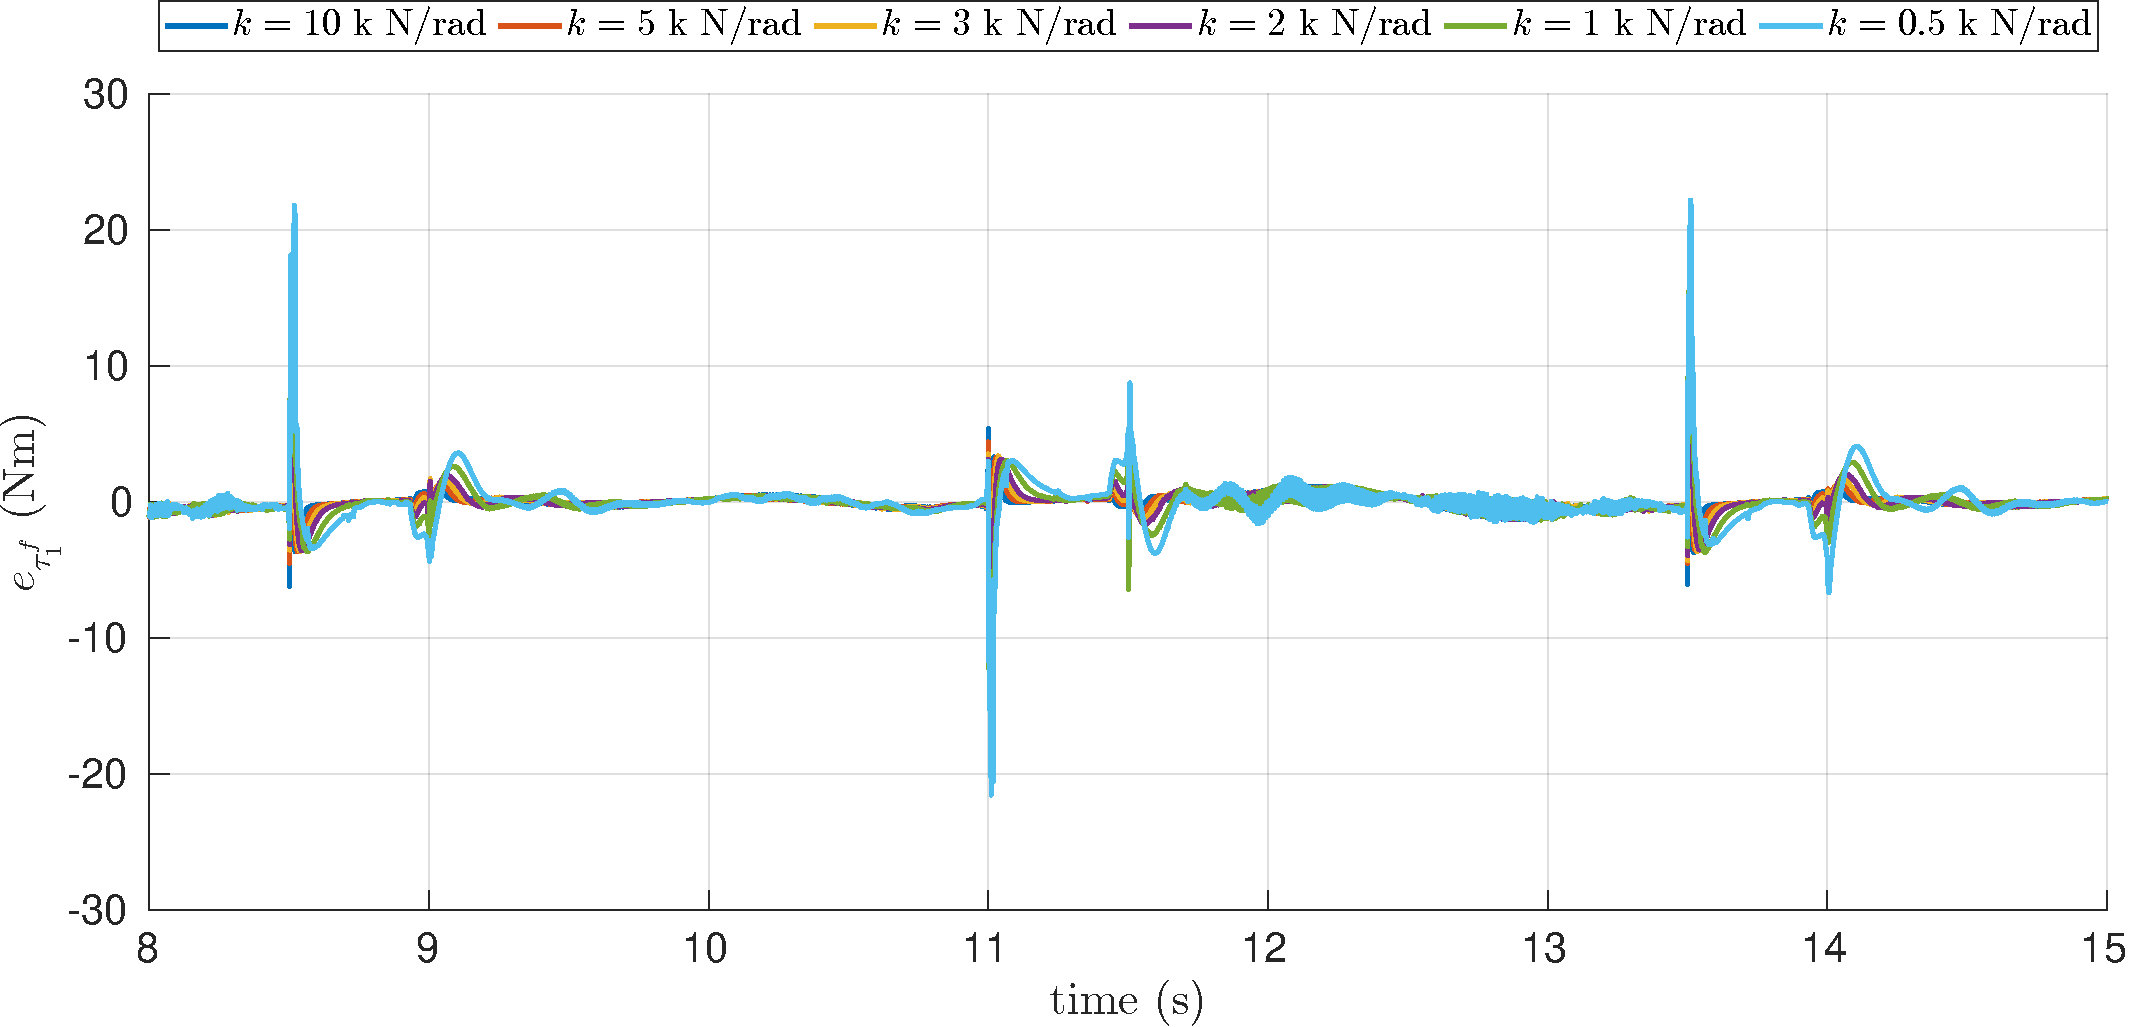
\includegraphics[width=\columnwidth]{chapter_flexible_joints/figures/estimation_left_tau_flex_1.pdf}
        \caption{Flexible joint torque error.\label{fig:flex_joint_trq_error}}
    \end{subfigure}
    \hfill
    \begin{subfigure}[b]{0.8\textwidth}
        \centering
        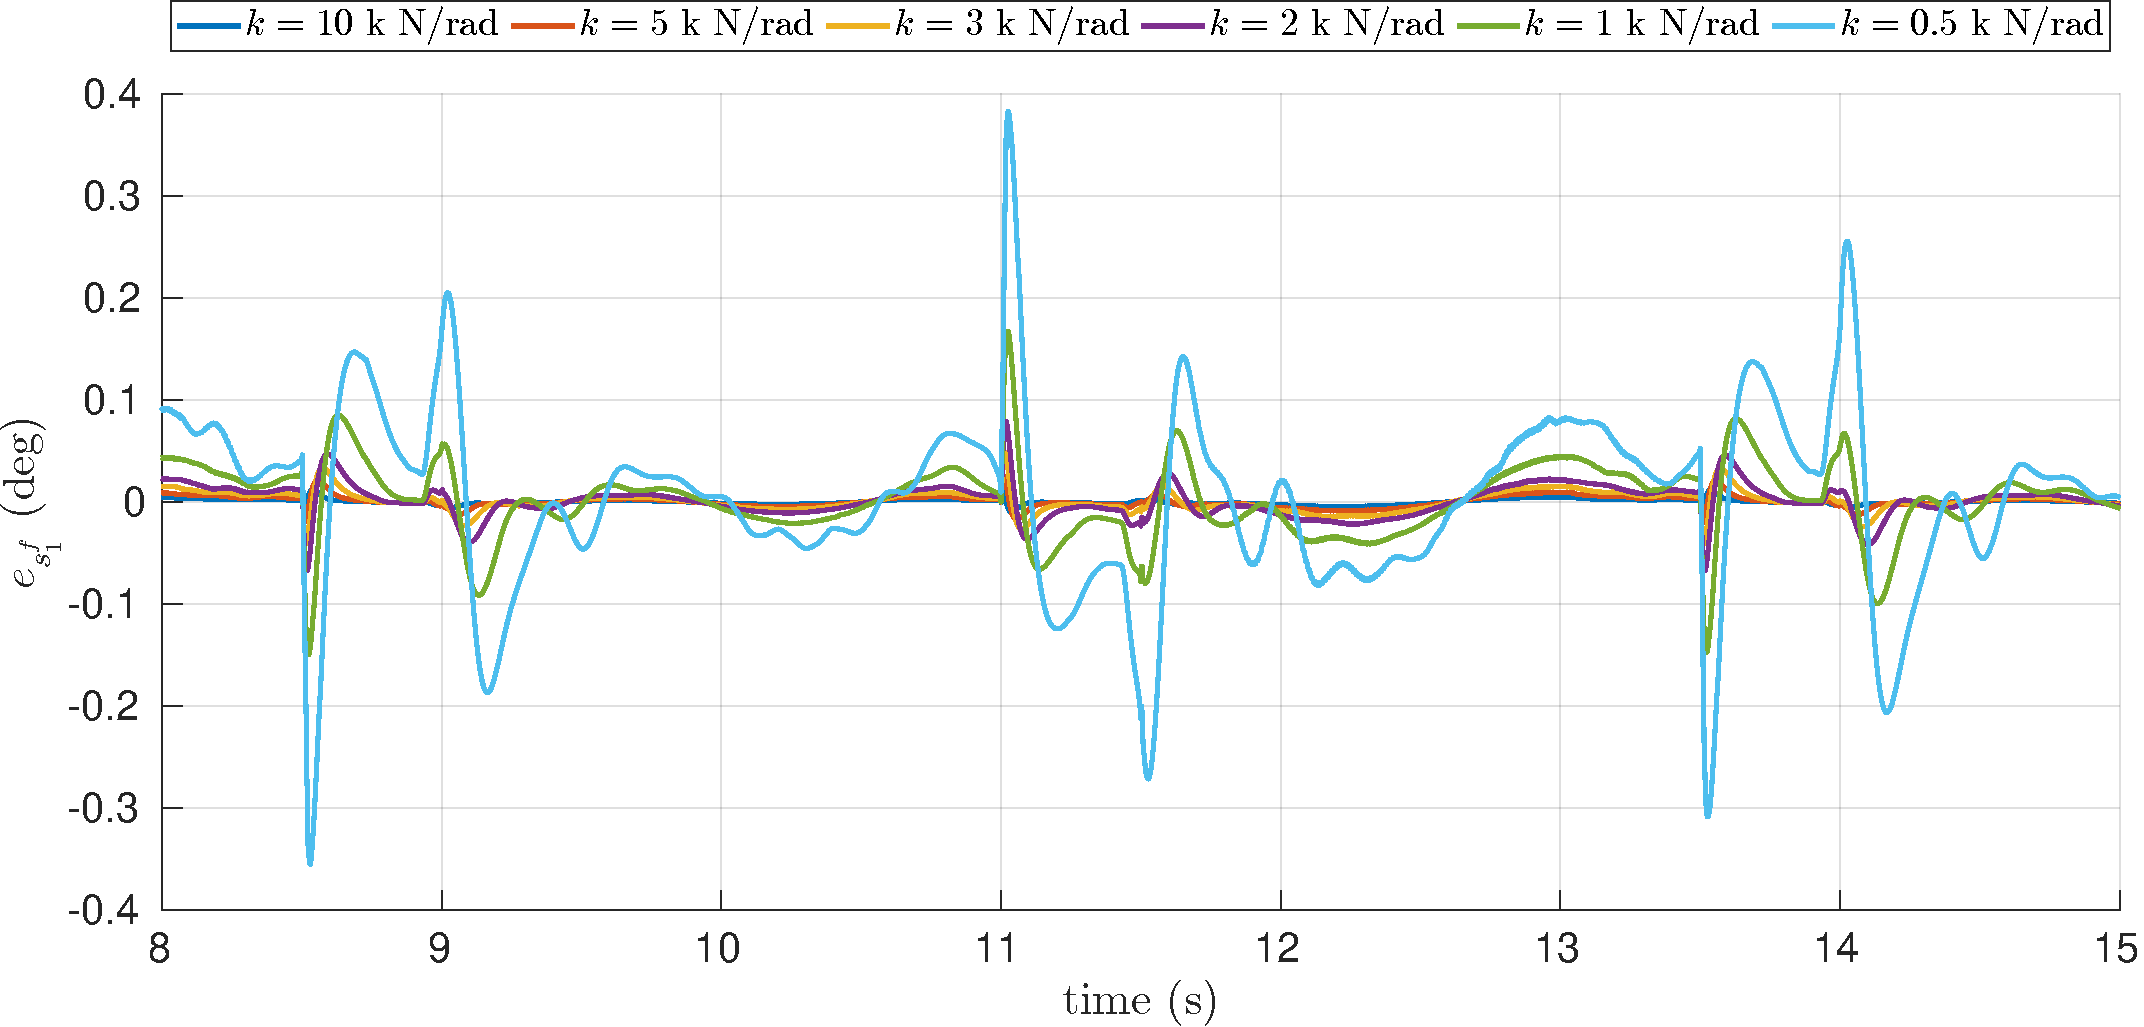
\includegraphics[width=\columnwidth]{chapter_flexible_joints/figures/estimation_left_q_flex_1.pdf}
        \caption{Flexible joint position error.\label{fig:flex_joint_pos_error}}
    \end{subfigure}
     \begin{subfigure}[b]{0.8\textwidth}
        \centering
        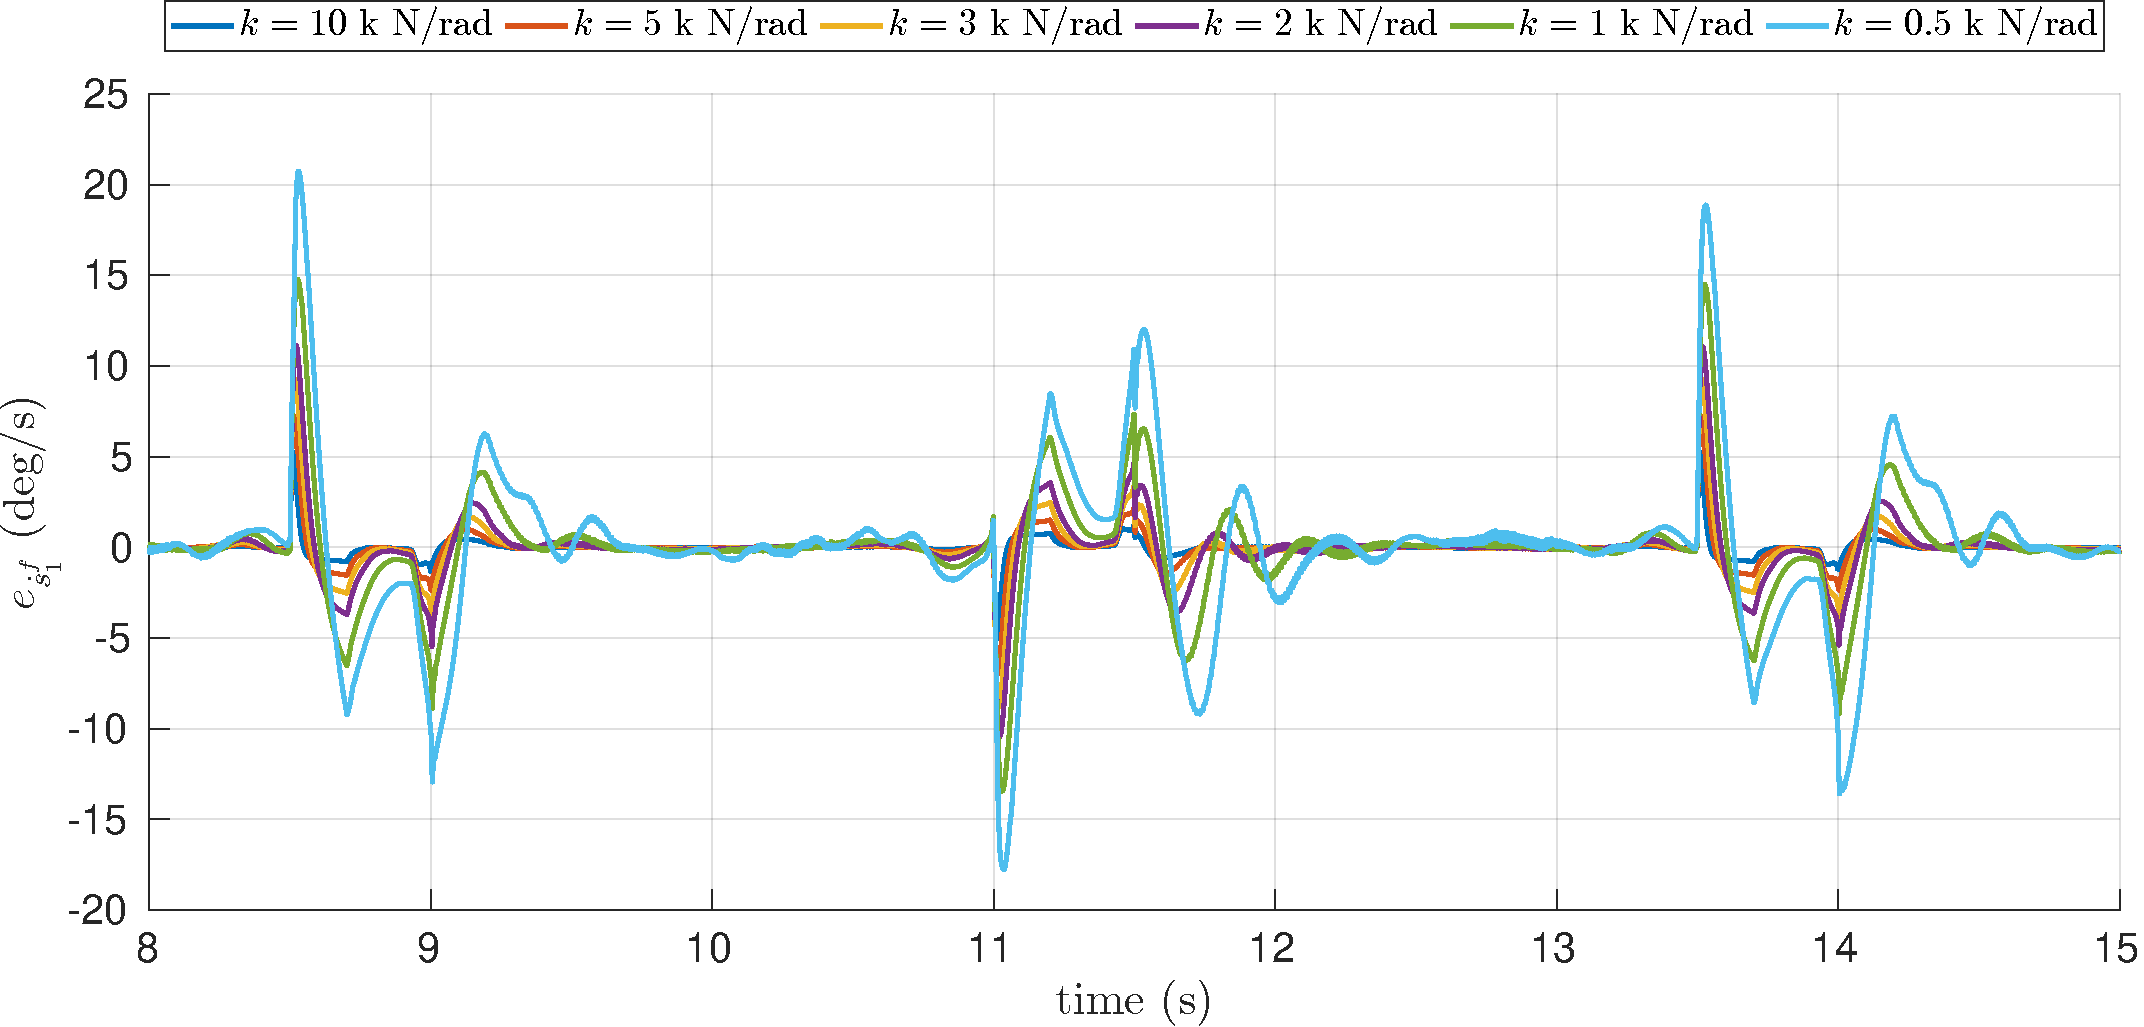
\includegraphics[width=\columnwidth]{chapter_flexible_joints/figures/estimation_left_dq_flex_1.pdf}
        \caption{Flexible joint velocity error.\label{fig:flex_joint_vel_error}}
    \end{subfigure}
    \end{myframe}
    \caption{Flexible joint state estimation error.\label{fig:estimation_flex_1}}
\end{figure}
Figure~\ref{fig:estimation_com_flex} shows the CoM tracking error for different values of $k$. The controller induces an acceptable performance for all values of $k$, i.e., the error is always below $\SI{3}{\milli\meter}$. However, the lower the stiffness, the higher the tracking error.  This increase in tracking error is caused by the flexible joint state estimation error.
Figure~\ref{fig:estimation_flex_1} presents the estimation error of a flexible joint. Similar considerations hold also for the other three joints. When the robot switches from single support to double support, the estimated torque associated with the flexible joint has a spike -- at $t\approx\SI{8.5}{\second}$, $\SI{11}{\second}$ and $\SI{13.5}{\second}$ in Figure~\ref{fig:flex_joint_trq_error}. As a consequence, the error propagates in the estimation of the flexible joint position and velocity -- see Figures~\ref{fig:flex_joint_pos_error} and~\ref{fig:flex_joint_vel_error}. This behavior is caused by the discontinuity of the contact force. To mitigate this effect, we may try to perform a smother transition from single to double support and vice versa.
The lower the stiffness parameter $k$, the higher the estimation error. 




